%=======================================================================
%  PE4 -- Practica Experimental Unidad IV
%  Ingenieria de Requerimientos (ISR-401) -- UTEQ
%  Equipo B: Mora Duarte, Rizzo Velez, Villafuerte Rosero
%
%  COMPILACION (tres pasadas obligatorias):
%     pdflatex PE4_U4_MORA_RIZZO_VILLAFUERTE
%     bibtex   PE4_U4_MORA_RIZZO_VILLAFUERTE
%     pdflatex PE4_U4_MORA_RIZZO_VILLAFUERTE
%     pdflatex PE4_U4_MORA_RIZZO_VILLAFUERTE
%
%  ANTES DE ENTREGAR: buscar "pendiente" en este archivo y eliminar
%  TODAS las marcas. Un solo marcador visible en el PDF activa el
%  indicador S2 de la escala DIA (andamiaje de plantilla sin completar).
%=======================================================================
\documentclass[11pt,letterpaper]{article}

\usepackage[utf8]{inputenc}
\usepackage[T1]{fontenc}
% Carga condicional: si la instalacion de LaTeX no incluye el modulo de espanol
% (paquete texlive-lang-spanish), el documento compila igual en lugar de abortar.
\IfFileExists{spanish.ldf}{\usepackage[spanish,es-tabla]{babel}}{}
\usepackage[margin=2.5cm]{geometry}
\usepackage{graphicx}
\usepackage{booktabs}
\usepackage{longtable}
\usepackage{array}
\usepackage{tabularx}
\usepackage{multirow}
\usepackage{xcolor}
\usepackage{caption}
\usepackage{float}
\usepackage{enumitem}
\usepackage{fancyhdr}
\usepackage{listings}
\usepackage{siunitx}
\usepackage{pgfplots}
\pgfplotsset{compat=1.18}
\usepackage[hidelinks]{hyperref}
\usepackage{xurl}
\setlength{\emergencystretch}{3em}
\graphicspath{{figuras/}}
\sisetup{output-decimal-marker={,}}

% --- Identificadores de requisito en versalitas monoespaciadas ---
\newcommand{\id}[1]{\texttt{#1}}

% --- Marcador de contenido pendiente (ELIMINAR ANTES DE ENTREGAR) ---
\newcommand{\pendiente}[1]{\textcolor{red}{\textbf{[PENDIENTE: #1]}}}

% --- Encabezado y pie ---
\pagestyle{fancy}
\fancyhf{}
\fancyhead[L]{\footnotesize PE4 --- Unidad IV: Validación y Gestión de Requisitos}
\fancyhead[R]{\footnotesize ISR-401 --- UTEQ}
\fancyfoot[C]{\footnotesize Página \thepage}
\renewcommand{\headrulewidth}{0.4pt}

\newcolumntype{L}[1]{>{\raggedright\arraybackslash}p{#1}}

\begin{document}

%=======================================================================
% 1. CARATULA
%=======================================================================
\begin{titlepage}
\centering
\vspace*{1cm}

{\large\textbf{UNIVERSIDAD TÉCNICA ESTATAL DE QUEVEDO}}\\[0.3cm]
{\normalsize Facultad de Ciencias de la Computación}\\[0.2cm]
{\normalsize Carrera de Software (Rediseño)}\\[1.5cm]

{\large\textbf{PRÁCTICA EXPERIMENTAL --- UNIDAD IV}}\\[0.5cm]
{\Large\textbf{Validación, Gestión de Requisitos y Herramientas CASE}}\\[0.4cm]
{\normalsize Inspección Fagan · Change Control Board · Trazabilidad en herramienta CASE · Línea base con Git}\\[1.5cm]

{\normalsize\textbf{Sistema del Proyecto Fin de Curso}}\\[0.2cm]
{\large SIMPA --- Sistema Inteligente de Mantenimiento de Palma Africana}\\[0.2cm]
{\footnotesize Base de trabajo: ERS/SRS del SIMPA, Entrega 2A (versión vigente)}\\[1.2cm]

{\normalsize\textbf{Integrantes y roles}}\\[0.4cm]
\begin{tabular}{L{5.5cm} L{4cm} L{4cm}}
\toprule
\textbf{Integrante} & \textbf{Rol en la inspección} & \textbf{Rol en el CCB}\\
\midrule
Mora Duarte Alex José & Lector & Representante del cliente\\
Rizzo Vélez Edson Nagib & Moderador e Inspector 2 & Presidente del CCB\\
Villafuerte Rosero Allan Noe & Inspector 1 & Analista y desarrollador\\
\bottomrule
\end{tabular}\\[1.2cm]

{\normalsize\textbf{Asignatura:} Ingeniería de Requerimientos (ISR-401) --- 4.\textsuperscript{o} nivel}\\[0.2cm]
{\normalsize\textbf{Docente:} Ing. Gleiston Cicerón Guerrero Ulloa, PhD}\\[0.2cm]
{\normalsize\textbf{Fecha:} Miercoles 5 de Agosto del 2026

{\normalsize\textbf{Repositorio del trabajo}}\\[0.2cm]
{\small\url{https://github.com/erizzov-boop/ISR401-PFC-ERS-EQUIPO_B}}\\[1.5cm]

{\footnotesize Quevedo --- Los Ríos --- Ecuador}

\end{titlepage}

\tableofcontents
\newpage

%=======================================================================
% 2. RESUMEN Y OBJETIVOS
%=======================================================================
\section{Resumen y objetivos}

\subsection*{Resumen}

Este informe documenta la aplicación de técnicas formales de validación y gestión de requisitos
sobre la Especificación de Requisitos de Software del SIMPA, sistema de gestión y diagnóstico
asistido del cultivo de palma africana desarrollado como Proyecto Fin de Curso. Se ejecutó una
inspección formal según el método de Fagan sobre el documento vigente, con roles diferenciados,
preparación individual previa y registro estructurado de defectos, del que se derivaron métricas de
densidad, distribución y tasa de detección. Los defectos de severidad crítica y mayor se corrigieron
y se documentaron con su texto antes y después. A partir de un conflicto detectado en la inspección
y de dos escenarios adicionales se tramitaron tres solicitudes formales de cambio, cuyo análisis de
impacto se derivó recorriendo la matriz de trazabilidad del proyecto y que fueron deliberadas y
decididas en una sesión simulada de Change Control Board. La trazabilidad bidireccional del ERS se
implementó en Jira mediante una estructura de épicas, historias y sub-tareas con campos
personalizados de prioridad y de fuente del requisito. La versión resultante del documento se
publicó como línea base mediante control de versiones, con commits semánticos, etiqueta anotada y
registro de cambios. El informe cierra con una comparativa argumentada de herramientas CASE de
ingeniería de requisitos, un contraste entre el enfoque documental y el enfoque ágil, y conclusiones
derivadas de los resultados obtenidos por el equipo.

\subsection*{Objetivo general}

Aplicar técnicas formales de validación de requisitos, gestionar cambios mediante un Change Control
Board simulado, implementar la trazabilidad del ERS en una herramienta CASE, establecer una línea
base con Git y comparar metodológicamente la ingeniería de requisitos tradicional frente a la ágil,
sobre el ERS real del SIMPA.

\subsection*{Objetivos específicos}

\begin{enumerate}[leftmargin=*]
  \item Ejecutar una inspección formal tipo Fagan sobre el ERS del SIMPA, con roles diferenciados,
        lista de verificación y registro de defectos.
  \item Calcular e interpretar las métricas de inspección: densidad de defectos, distribución por
        tipo y severidad, tasa de detección por inspector y esfuerzo en horas-persona.
  \item Tramitar tres solicitudes formales de cambio con análisis de impacto sustentado en la matriz
        de trazabilidad.
  \item Deliberar y decidir en un CCB simulado, dejando acta motivada y versión actualizada del ERS.
  \item Construir la trazabilidad bidireccional del ERS en Jira, con campos personalizados y enlaces
        verificables.
  \item Establecer y publicar la línea base del ERS mediante commit semántico, etiqueta anotada y
        registro de cambios.
  \item Comparar herramientas CASE de ingeniería de requisitos y contrastar el enfoque tradicional
        frente al ágil.
\end{enumerate}

%=======================================================================
% 3. FUNDAMENTO TEORICO
%=======================================================================
\section{Fundamento teórico}

\subsection{Marco normativo}

La validación de requisitos no es una actividad discrecional del equipo de desarrollo sino un
proceso definido en la normativa internacional. La norma ISO/IEC/IEEE 29148:2018 ubica la validación
de requisitos en su cláusula 6.4, donde establece que el conjunto de requisitos debe demostrarse
completo, consistente y verificable antes de servir de base al diseño, y donde se enumeran las
propiedades que todo requisito individual debe satisfacer: necesidad, adecuación, ausencia de
ambigüedad, completitud, singularidad, factibilidad, verificabilidad, corrección y conformidad
\cite{iso29148}. Estas nueve propiedades constituyen el criterio operativo con el que se construyó
la lista de verificación del Anexo A de esta práctica.

Los procesos de control de cambios se definen en el nivel de ciclo de vida. La norma
ISO/IEC/IEEE 15288:2023 sitúa la gestión de la configuración entre los procesos técnicos de gestión
del proyecto y establece que todo elemento de configuración debe someterse a control de cambios una
vez incorporado a una línea base \cite{iso15288}. La norma ISO/IEC/IEEE 12207:2017 desarrolla el
mismo proceso para el ciclo de vida del software, con las actividades de identificación,
control, contabilidad de estado y auditoría de la configuración \cite{iso12207}. La consecuencia
práctica para esta práctica es directa: el ERS solo puede modificarse mediante solicitudes formales
de cambio una vez publicada la línea base, y toda modificación debe quedar registrada con su
autoridad aprobatoria.

El modelo de calidad de producto de ISO/IEC 25010:2023 aporta el vocabulario con el que se
especifican y evalúan los requisitos no funcionales. Su revisión de 2023 reorganiza el modelo en
nueve características, incorpora la seguridad física (\emph{safety}) como característica de primer
nivel y sustituye la portabilidad por la flexibilidad, de la que aquella pasa a ser
subcaracterística \cite{iso25010}. Esta precisión de versiones no es un detalle editorial: como se
documenta en la sección \ref{sec:inspeccion}, la inspección detectó que el ERS del SIMPA declara
cubrir las nueve características de la edición 2023 mientras emplea la taxonomía de la edición
anterior.

El cuerpo de conocimiento SWEBOK v4.0 dedica las secciones 1.6 a 1.8 de su área de requisitos a la
validación, la gestión y las consideraciones prácticas, y describe la inspección, el prototipado y
la validación de modelos como las técnicas centrales de comprobación \cite{swebok4}. Pohl desarrolla
la validación como una de las tres actividades nucleares de la ingeniería de requisitos, junto con
la elicitación y la documentación, y sistematiza los principios y las técnicas que la componen
\cite{pohl2025}. Finalmente, la séptima edición del PMBOK describe el Change Control Board como el
órgano formalmente constituido que revisa, evalúa, aprueba, difiere o rechaza los cambios de un
proyecto, y que registra sus decisiones \cite{pmbok7}; el sílabo IREB CPRE de nivel fundamental
aporta la terminología de gestión y trazabilidad empleada en este informe \cite{ireb31}.

\subsection{Validación de requisitos}

\subsubsection*{Verificación frente a validación}

La distinción entre ambos conceptos es la fuente más frecuente de confusión terminológica. La
verificación responde a la pregunta de si el documento se construyó correctamente, es decir, si
cumple las reglas de forma, completitud y consistencia interna que le son exigibles. La validación
responde a la pregunta de si el documento describe el sistema que las partes interesadas
efectivamente necesitan \cite{pohl2025}. Un ERS puede estar verificado y no validado: sus requisitos
pueden ser individualmente correctos, no ambiguos y trazables, y aun así especificar un sistema que
no resuelve el problema del cliente. Una inspección formal opera predominantemente en el plano de la
verificación, pero incorpora validación en la medida en que confronta cada requisito con la
evidencia de campo que lo origina.

\subsubsection*{Principios de validación}

Pohl formula seis principios que gobiernan la actividad \cite{pohl2025}: la participación de las
partes interesadas correctas, la separación entre la detección y la corrección de errores, la
validación desde múltiples perspectivas, el uso de documentación adecuada al perfil del validador,
la construcción de artefactos de desarrollo como medio de validación, y la repetición de la
validación tras cada cambio relevante. El segundo principio es el que determina la mecánica de la
reunión de inspección: discutir soluciones durante la sesión reduce la tasa de detección, porque
desvía la atención del grupo del documento hacia el diseño.

\subsubsection*{Técnicas de validación}

Las técnicas de comprobación se ordenan por grado de formalidad. La \emph{revisión informal} consiste
en la lectura por un colega sin proceso definido; es barata y de baja tasa de detección. El
\emph{walkthrough} es una presentación conducida por el autor ante un grupo, orientada a la
comprensión compartida más que a la medición. La \emph{inspección} es el extremo formal: proceso
definido, roles diferenciados, preparación individual obligatoria, criterios de entrada y salida, y
registro cuantificado de defectos. A ellas se suman el \emph{prototipado}, que valida mediante la
construcción de un artefacto ejecutable; las \emph{listas de verificación}, que sistematizan las
propiedades a comprobar; y la \emph{validación por perspectivas}, en la que cada revisor adopta el
punto de vista de una parte interesada distinta \cite{pohl2025, swebok4}.

\subsubsection*{El método de Fagan}

Fagan formalizó la inspección en el desarrollo de software del System/370 de IBM y reportó
reducciones de defectos superiores al veinte por ciento respecto de los métodos de revisión
entonces vigentes \cite{fagan1976}. El método define seis fases: planificación, en la que se verifica
que el documento cumple los criterios de entrada y se asignan los roles; visión general
(\emph{overview}), en la que el autor presenta el material; preparación individual, en la que cada
inspector examina el documento por separado; reunión de inspección, en la que se consolidan los
defectos; retrabajo, en el que el autor corrige; y seguimiento, en el que el moderador verifica que
las correcciones se aplicaron.

Los cuatro roles son igualmente característicos. El \emph{moderador} conduce la sesión, controla el
tiempo y consolida el registro. El \emph{lector} parafrasea el documento sección por sección, y la
paráfrasis es deliberada: leer literalmente permitiría que el grupo reprodujera la misma
interpretación errónea del autor, mientras que reformular obliga a explicitar el significado
atribuido y expone las ambigüedades. Los \emph{inspectores} reportan los defectos preparados. La
regla operativa que atraviesa todo el método es que la inspección detecta pero no corrige.

\subsubsection*{Métricas de inspección}

El valor del método reside tanto en los defectos que encuentra como en los datos que produce. Las
métricas empleadas en esta práctica son la densidad de defectos (defectos detectados por página
efectiva inspeccionada), la distribución por tipo, la distribución por severidad, la tasa de
detección por inspector y el esfuerzo total en horas-persona. Su interpretación no es mecánica: una
densidad elevada puede indicar un documento deficiente o una inspección eficaz, y solo el contraste
con la distribución por tipo permite distinguir ambos casos.

\subsubsection*{Ejemplo aplicado}

En la inspección documentada en la sección \ref{sec:inspeccion}, la concentración de defectos en la
propiedad de consistencia --- y específicamente en los conteos de requisitos declarados en distintas
secciones del mismo documento --- resultó atribuible a un patrón identificable: el ERS del SIMPA
creció por acumulación de entregas sucesivas, y las secciones agregadas en la última iteración no
propagaron sus efectos a las secciones heredadas. Es el mismo fenómeno que Wiegers describe como
deriva de consistencia en documentos versionados sin revisión integral \cite{wiegers2013}.

\subsection{Gestión de requisitos}

\subsubsection*{Configuración, línea base y versionado}

Una línea base es un conjunto de requisitos formalmente revisado y acordado que sirve de referencia
para el desarrollo posterior y que solo puede modificarse mediante un procedimiento de control de
cambios establecido \cite{iso12207, wiegers2013}. La distinción respecto de una simple versión es
sustantiva: cualquier guardado produce una versión, pero solo un acto de aprobación produce una
línea base. En esta práctica esa aprobación la emite el CCB y su materialización técnica es la
etiqueta anotada de Git, que fija de forma inmutable el estado del repositorio aprobado.

\subsubsection*{Atributos de requisitos}

La gestión exige que cada requisito lleve asociados atributos que permitan filtrarlo, priorizarlo y
seguirlo: identificador único, versión, autor, fuente, prioridad, estado, criterio de aceptación,
esfuerzo estimado y responsable \cite{iso29148, wiegers2013}. Los campos personalizados configurados
en Jira, descritos en la sección \ref{sec:trazabilidad}, son la implementación de este concepto sobre
una herramienta concreta.

\subsubsection*{Trazabilidad}

Gotel y Finkelstein establecieron la distinción que sigue estructurando el campo: la
\emph{pre-trazabilidad} vincula el requisito con su origen anterior a la especificación --- la parte
interesada, el documento fuente, la sesión de elicitación ---, mientras que la
\emph{post-trazabilidad} lo vincula con los artefactos derivados de él \cite{gotel1994}. Sobre ese eje
se superpone la dirección: la trazabilidad hacia atrás permite responder por qué existe un
requisito, y la trazabilidad hacia adelante permite determinar qué se ve afectado si el requisito
cambia. Solo la combinación de ambas hace posible el análisis de impacto; una matriz que enlaza
únicamente hacia adelante permite estimar el costo de un cambio pero no justificar su rechazo ante
la parte interesada que lo solicitó \cite{clelandhuang2012}.

La matriz de trazabilidad es el artefacto que materializa estos enlaces. Un requisito sin enlace
hacia atrás es huérfano y su necesidad no puede justificarse; un requisito sin enlace hacia adelante
no está implementado ni probado y constituye un vacío de cobertura.

\subsubsection*{El proceso de cambio}

El ciclo formal comprende cinco etapas \cite{pmbok7, wiegers2013}. La \emph{solicitud} se registra en
un formulario de cambio con solicitante, requisito afectado, descripción y justificación de negocio.
El \emph{análisis de impacto} recorre la matriz de trazabilidad para identificar los requisitos y
artefactos afectados de forma directa e indirecta, estima el esfuerzo y evalúa el riesgo; su calidad
depende enteramente de que el recorrido sea sistemático y no una estimación a ojo. La \emph{decisión}
corresponde al CCB, que aprueba, aprueba con condiciones, difiere o rechaza, y que debe motivar la
decisión. La \emph{implementación} aplica el cambio y actualiza la versión del documento. El
\emph{cierre} verifica la aplicación y publica la nueva línea base.

\subsubsection*{Volatilidad de requisitos}

La volatilidad mide la tasa de cambio del conjunto de requisitos por unidad de tiempo o por fase, y
suele expresarse como el cociente entre requisitos añadidos, modificados y eliminados sobre el total
de la línea base \cite{wiegers2013}. Una volatilidad alta en fases tardías es un predictor conocido
de desviación de plazo y de costo, y su medición proporciona al CCB el argumento cuantitativo para
diferir cambios no críticos.

\subsection{Herramientas CASE para ingeniería de requisitos}

Las herramientas CASE se clasifican tradicionalmente según la fase del ciclo de vida que soportan.
Las \emph{upper CASE} asisten las fases tempranas ---análisis, especificación y modelado---; las
\emph{lower CASE} asisten la implementación, la generación de código y las pruebas; y las
\emph{integrated CASE} o \emph{I-CASE} cubren el ciclo completo con un repositorio común
\cite{swebok4}. Las herramientas de gestión de requisitos pertenecen a la primera categoría, aunque
las plataformas contemporáneas tienden a la integración mediante conectores.

Las funcionalidades esperables de una herramienta de gestión de requisitos son seis: un
\emph{repositorio} único que evite la dispersión en documentos ofimáticos; \emph{atributos}
configurables por requisito; \emph{trazabilidad} bidireccional con visualización de matriz y análisis
de impacto; \emph{baselining}, es decir, capacidad de congelar y comparar versiones del conjunto;
\emph{control de cambios} con flujo de aprobación; y \emph{colaboración} con integración al sistema
de control de versiones y a la cadena de construcción \cite{wiegers2013, clelandhuang2012}.

Los criterios de selección deben ponderar, además de la funcionalidad, el costo total de propiedad,
la curva de aprendizaje del equipo, la disponibilidad de licencias académicas o gratuitas y la
capacidad de exportación de los datos, que determina la reversibilidad de la decisión. Las
limitaciones más frecuentes son el costo de las suites especializadas, la rigidez de sus modelos de
datos y el hecho de que ninguna herramienta suple la ausencia de un proceso: una herramienta de
gestión de requisitos usada como lista de tareas produce un tablero, no trazabilidad.

\subsection{Ingeniería de requisitos en procesos ágiles}

En los marcos ágiles el ERS documental se sustituye por un \emph{product backlog} priorizado y
emergente, en el que los requisitos se expresan como historias de usuario. Cohn propone el formato
que se ha vuelto canónico --- rol, funcionalidad, beneficio --- y los criterios INVEST, que exigen
que una historia sea independiente, negociable, valiosa, estimable, pequeña y verificable
\cite{cohn2004}. Los \emph{criterios de aceptación} completan la historia con las condiciones
observables de satisfacción, y son el equivalente funcional del criterio de verificación de un
requisito documental.

El refinamiento continuo del backlog (\emph{grooming}) y las definiciones de preparado
(\emph{Definition of Ready}) y de terminado (\emph{Definition of Done}) cumplen el papel que en el
enfoque documental desempeñan los criterios de entrada y salida de una inspección: establecen cuándo
un elemento está suficientemente especificado para entrar en desarrollo y cuándo puede considerarse
completo.

El desarrollo guiado por comportamiento (BDD) extiende esta lógica al hacer del criterio de
aceptación un artefacto ejecutable. El formato Gherkin --- \emph{Dado}, \emph{cuando},
\emph{entonces} --- expresa el escenario en lenguaje natural estructurado y permite su vinculación
directa con pruebas automatizadas \cite{smart2014}. El ERS del SIMPA emplea este formato en los
criterios de aceptación de sus historias, lo que constituye un caso de hibridación entre ambos
enfoques.

La trazabilidad en entornos ágiles es el punto de mayor tensión. La documentación ligera y la
priorización emergente dificultan mantener enlaces persistentes, y la práctica habitual la resuelve
mediante convenciones sobre los identificadores en los mensajes de commit y en las ramas, y mediante
la vinculación entre elementos del backlog y solicitudes de incorporación de código
\cite{clelandhuang2012}. El contraste con el enfoque documental se desarrolla en la
sección \ref{sec:comparativa}: no se trata de determinar cuál enfoque es superior, sino en qué
contextos --- criticidad, exigencia regulatoria, estabilidad del dominio, tamaño del equipo --- cada
uno resulta apropiado.

%=======================================================================
% 4. INSPECCION FAGAN
%=======================================================================
\section{Inspección formal del ERS (método Fagan)}
\label{sec:inspeccion}

\subsection{Planificación, roles y alcance}

\begin{table}[H]
\centering
\caption{Asignación de roles de la inspección}
\begin{tabular}{L{4.5cm} L{3.5cm} L{5cm}}
\toprule
\textbf{Integrante} & \textbf{Rol} & \textbf{Responsabilidad}\\
\midrule
Rizzo Vélez Edson Nagib & Moderador & Conduce la sesión, controla el tiempo y consolida el Anexo B\\
Mora Duarte Alex José & Lector & Parafrasea el documento sección por sección\\
Villafuerte Rosero Allan Noe & Inspector 1 & Prepara y reporta defectos\\
Rizzo Vélez Edson Nagib & Inspector 2 & Prepara y reporta defectos\\
\bottomrule
\end{tabular}
\end{table}

\noindent\textbf{Documento inspeccionado:} ERS/SRS del SIMPA v3.0, Entrega 2A, compilado desde las fuentes
\LaTeX{} versionadas en \texttt{01\_ERS/}.\\
\textbf{Secciones incluidas en el alcance:} \S1 a \S7 del ERS. Se excluyen los apéndices A--E.\\
\textbf{Páginas efectivas inspeccionadas:} 63 (pp. 8--70). La \S1 comienza en la página 8 y el
Apéndice~A en la 71; las siete primeras páginas corresponden a portada, historial de versiones e
índices, que no contienen requisitos y por tanto no se inspeccionan.\\
\textbf{Fecha y hora de la reunión:} Miercoles 5 de Agosto, 8:00 am - 9:30 am. \textbf{Duración:} {90 minutos}.

\vspace{0.2cm}
\noindent\fbox{\parbox{0.96\textwidth}{\small\textbf{Declaración sobre el criterio de admisión A3.}
La guía exige que los cuatro roles de la inspección correspondan a personas distintas. El equipo B
está integrado por tres personas, de modo que la exigencia no puede satisfacerse literalmente. Se
resuelve acumulando en un mismo integrante los roles de Moderador e Inspector~2, y se declara de
forma expresa en lugar de simular un cuarto participante. La acumulación recae sobre el Moderador
porque es el rol cuya función --- conducir y consolidar --- es compatible con haber realizado
preparación individual previa, mientras que separar a los dos inspectores preserva la independencia
de las dos lecturas críticas del documento. Las métricas de detección por inspector se reportan por
rol, no por persona, y el rol acumulado se identifica como tal en la Tabla~\ref{tab:preparacion}.}}

\subsection{Preparación individual}

Cada inspector recorrió el documento de forma independiente y completó su propia copia de la lista
de verificación del Anexo A sobre las seis propiedades evaluadas: ambigüedad, completitud,
consistencia, verificabilidad, trazabilidad y factibilidad. Las copias firmadas y fechadas se
encuentran en \texttt{02\_Inspeccion/AnexoA\_checklists/}.

\begin{table}[H]
\centering
\caption{Preparación individual por inspector}\label{tab:preparacion}
\begin{tabular}{L{4.5cm} L{2.6cm} L{2.6cm} L{3cm}}
\toprule
\textbf{Inspector} & \textbf{Defectos preparados} & \textbf{Horas-persona} & \textbf{Marca temporal}\\
\midrule
Rizzo Vélez (Moderador / Inspector 2) & {18} & {4} & {05/08/2026}\\
Mora Duarte (Lector) & 7} & {2} & {05/08/2026}\\
Villafuerte Rosero (Inspector 1) & {8} & {2} & {05/08/2026}\\
\bottomrule
\end{tabular}
\end{table}

\subsection{Acta de la reunión de inspección}

\begin{figure}
    \centering
    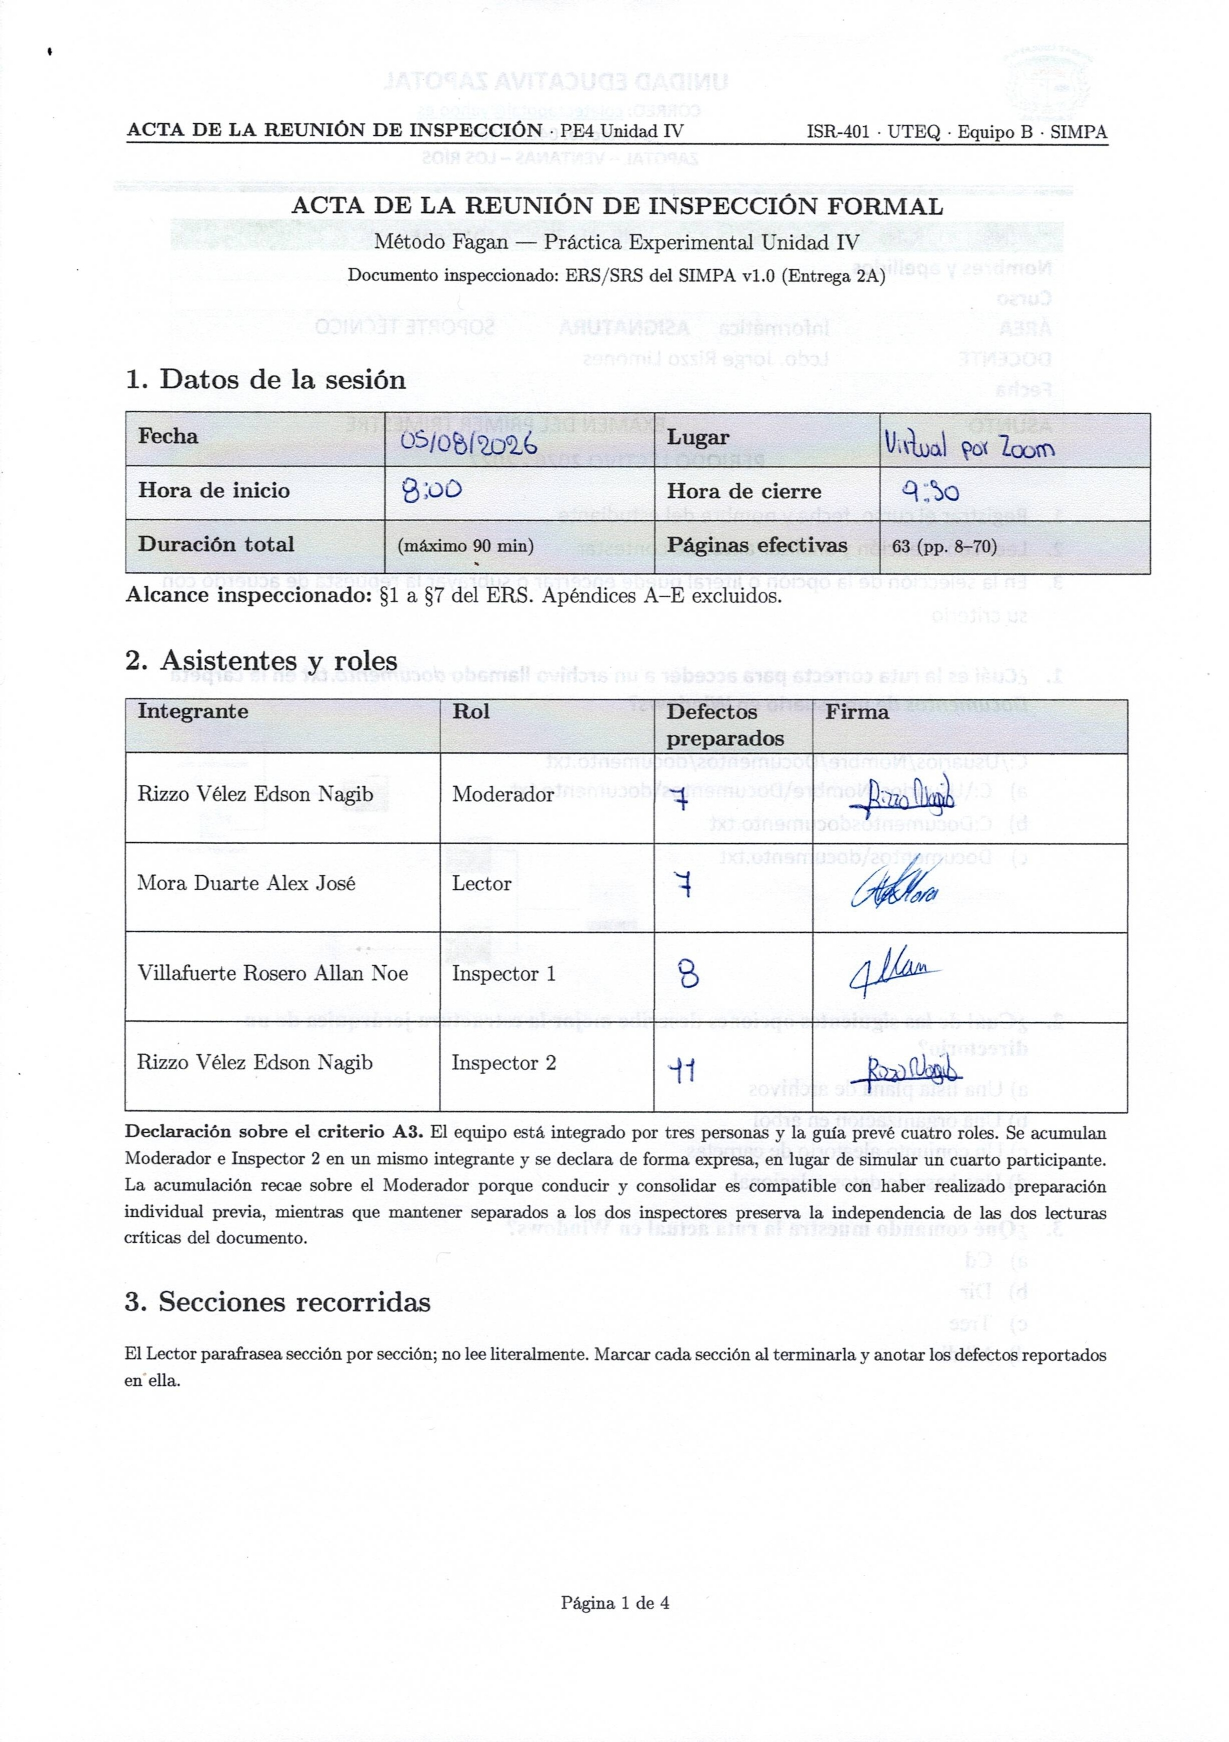
\includegraphics[width=0.5\linewidth]{Acta de la reunión de inspección formal 1.jpg}
    \caption{Acta de la reunión de inspección formal 1}
    \label{fig:placeholder}
\end{figure}

\begin{figure}
    \centering
    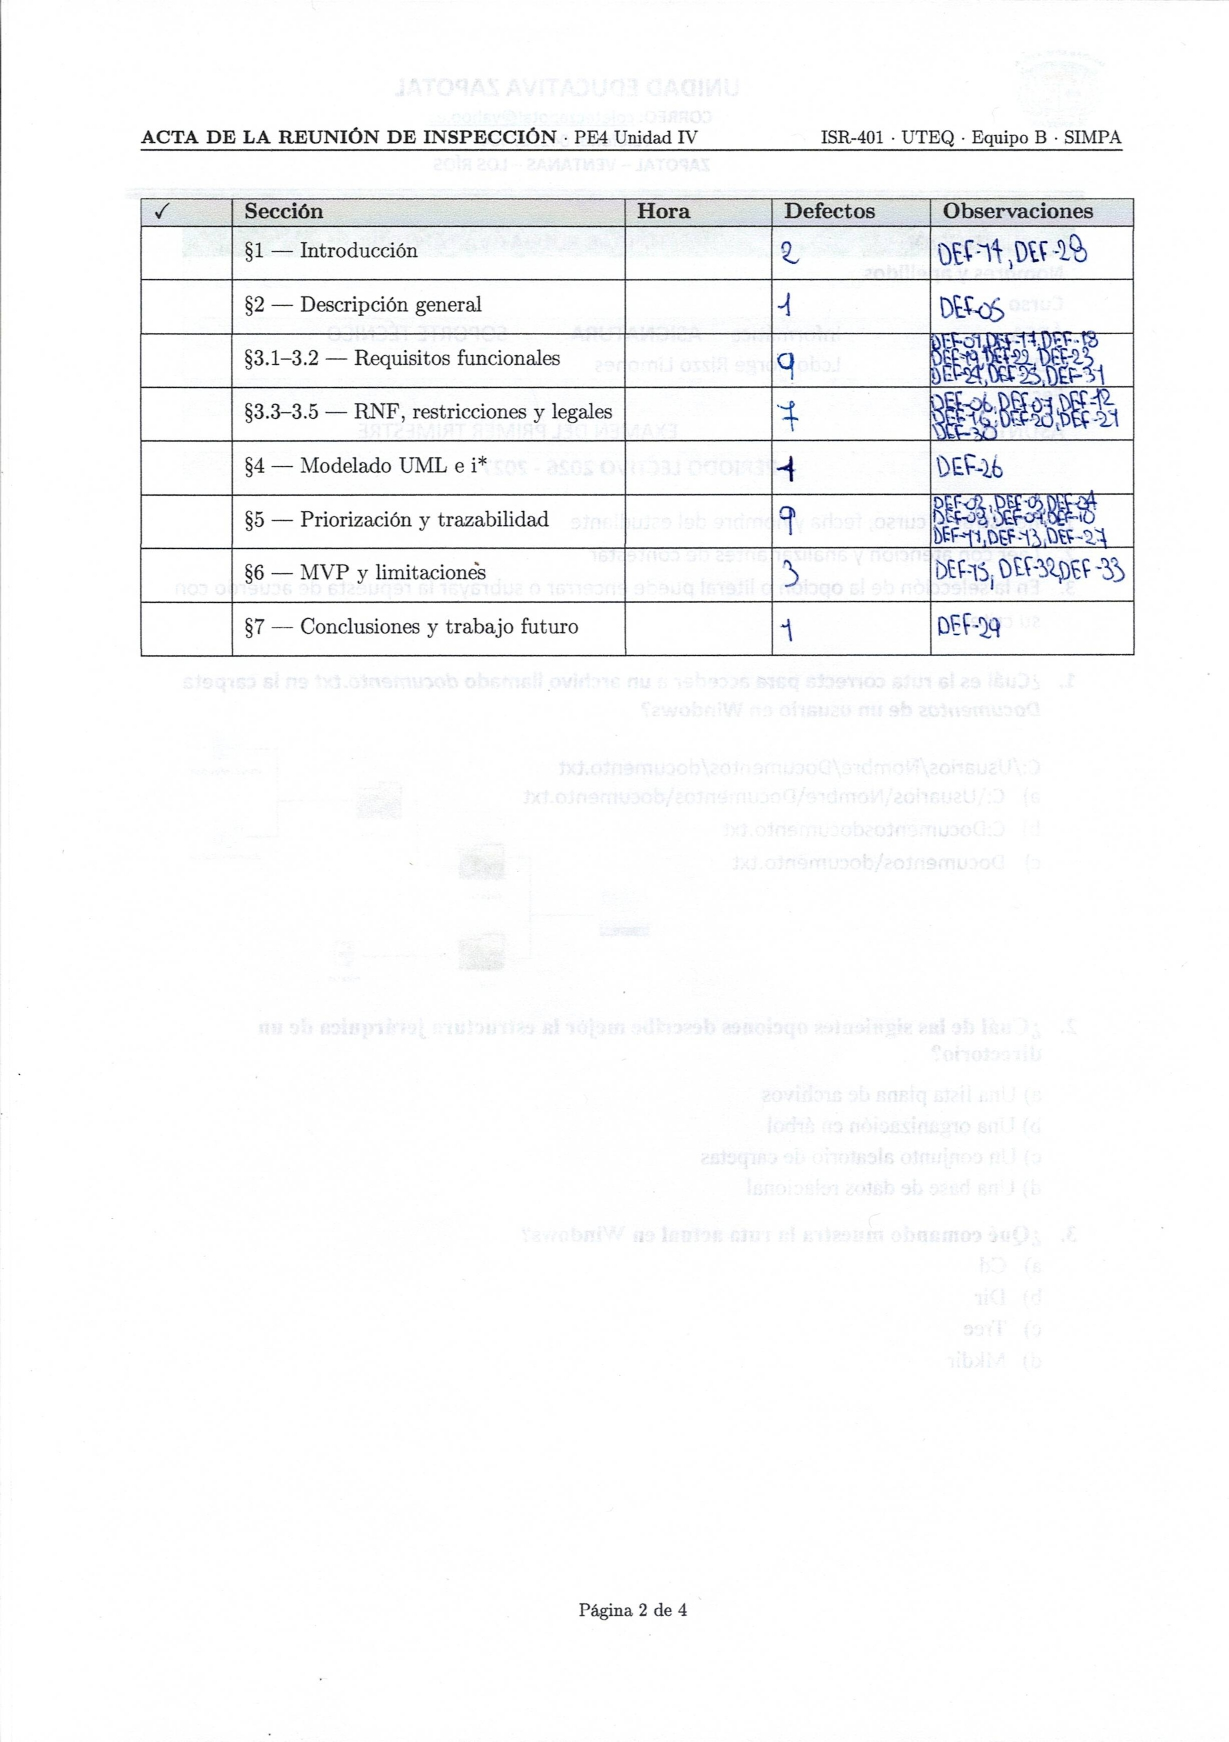
\includegraphics[width=0.5\linewidth]{Acta de la reunión de inspección formal 2.jpg}
    \caption{Acta de la reunión de inspección formal 2}
    \label{fig:placeholder}
\end{figure}

\begin{figure}
    \centering
    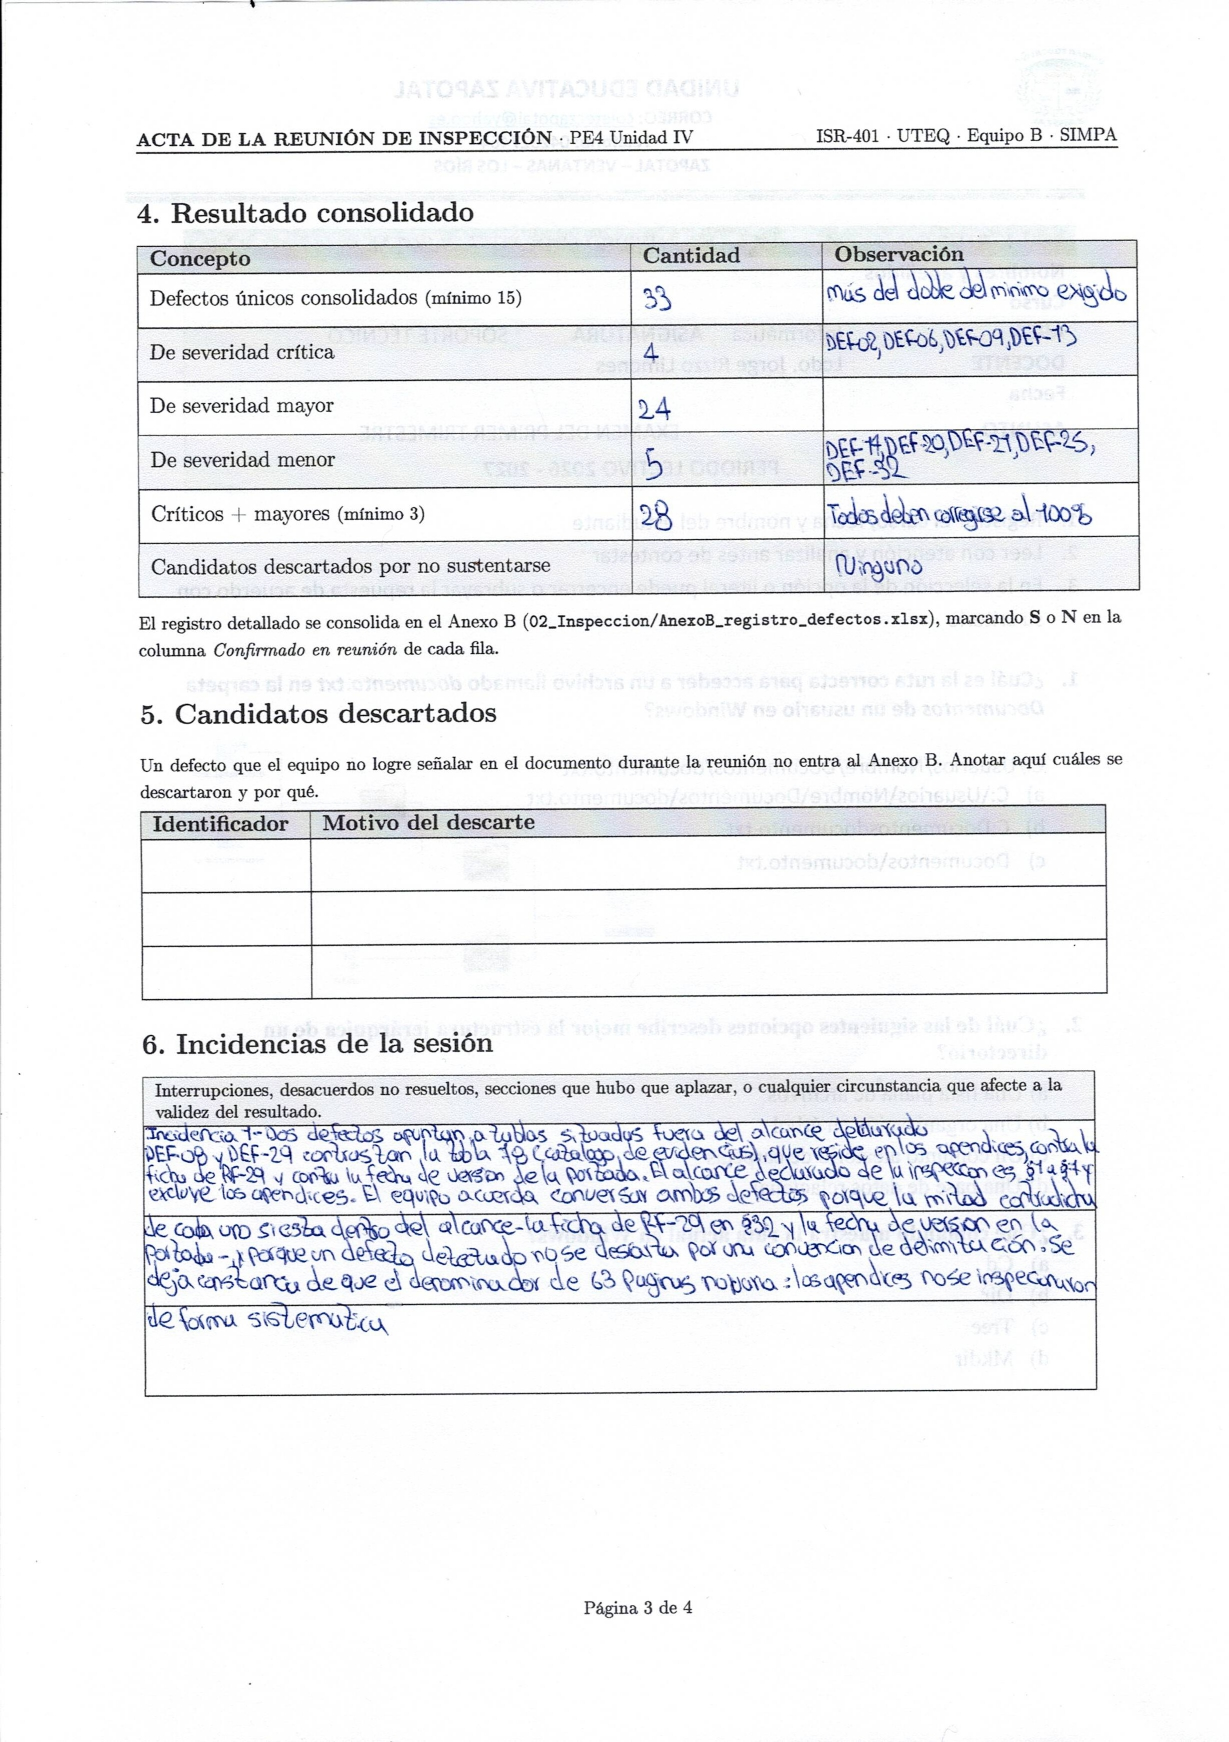
\includegraphics[width=0.5\linewidth]{Acta de la reunión de inspección formal 3.jpg}
    \caption{Acta de la reunión de inspección formal 3}
    \label{fig:placeholder}
\end{figure}

\begin{figure}
    \centering
    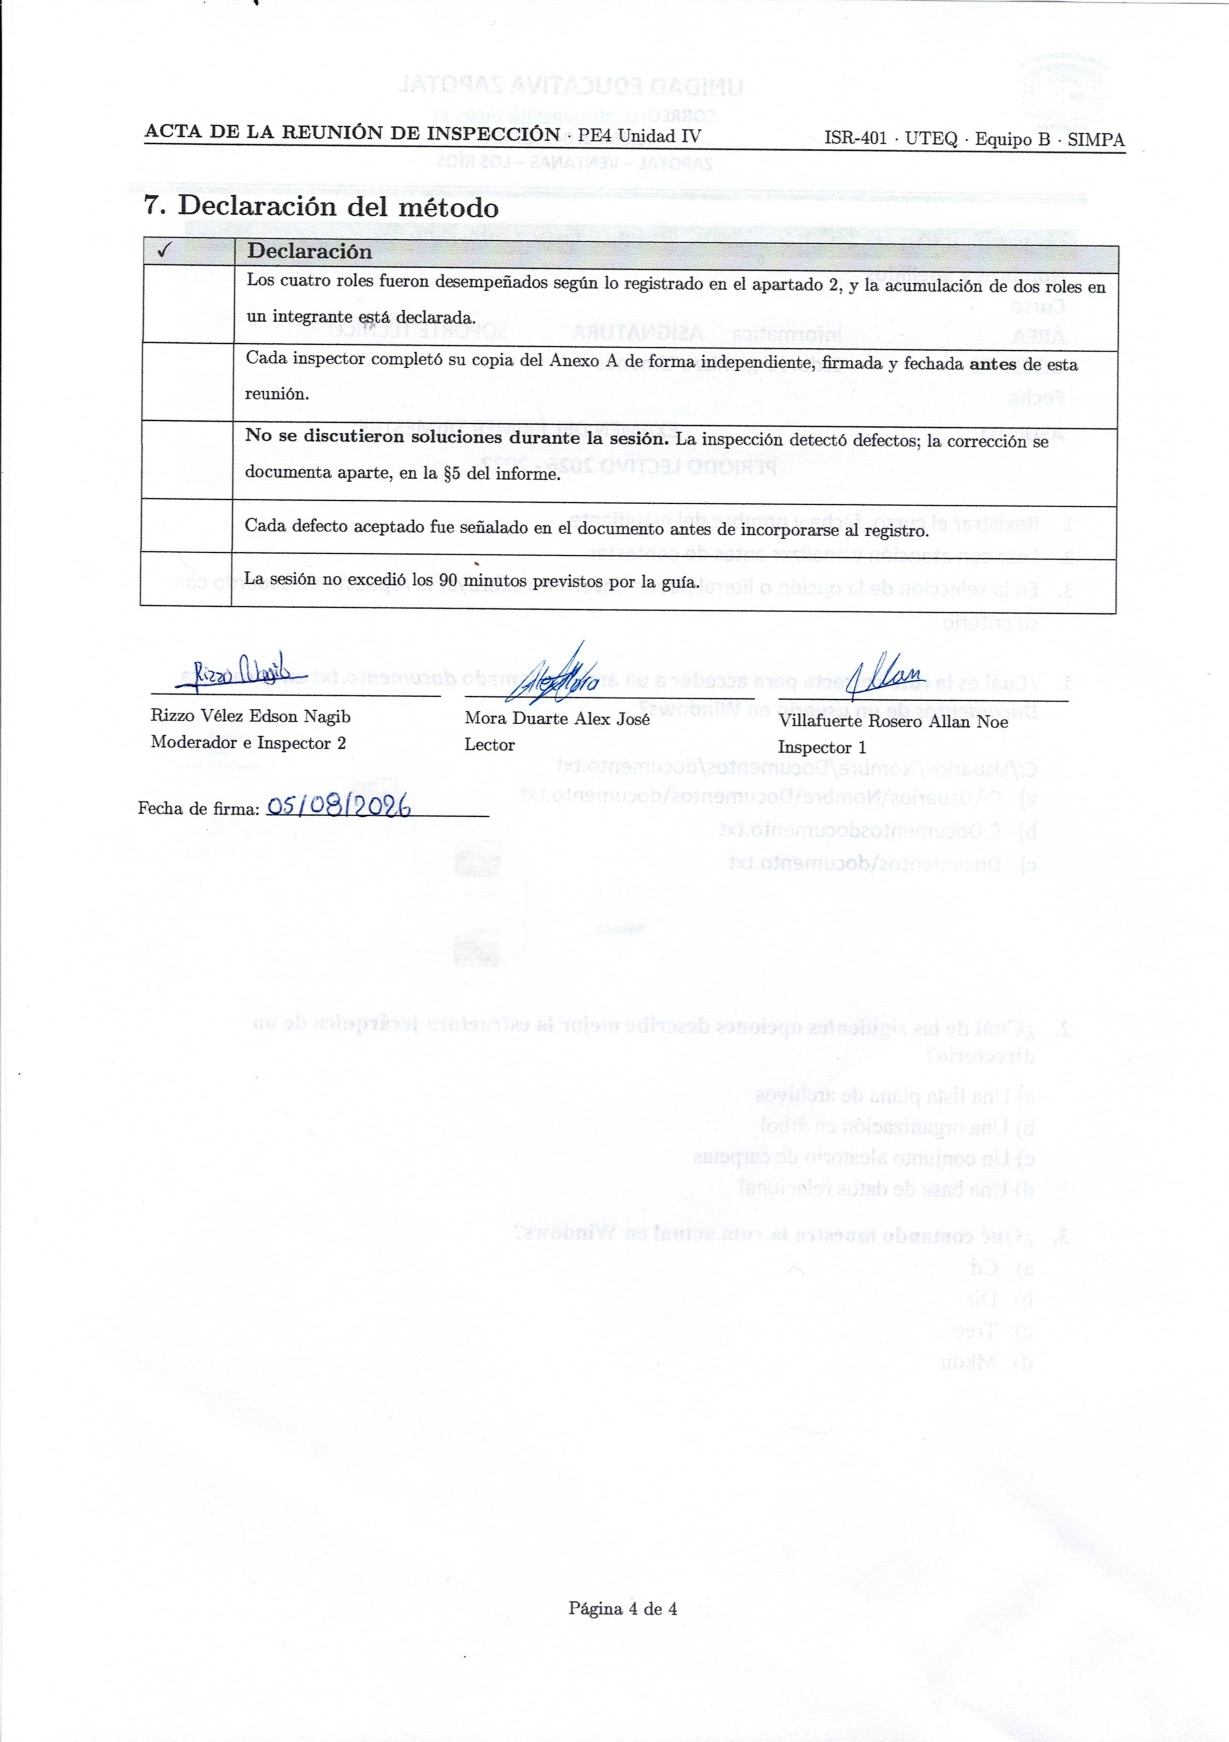
\includegraphics[width=0.5\linewidth]{Acta de la reunión de inspección formal 4.jpg}
    \caption{Acta de la reunión de inspección formal 4}
    \label{fig:placeholder}
\end{figure}

\subsection{Registro consolidado de defectos}

El registro completo constituye el Anexo B y se versiona en el archivo
\path{02_Inspeccion/AnexoB_registro_defectos.xlsx}. La tabla siguiente reproduce el consolidado:
33 defectos únicos, de los cuales 4 son de severidad crítica y 24 mayor, muy por encima del mínimo
exigido de 15 defectos con al menos 3 críticos o mayores.

Los defectos se identifican como \texttt{DEF-01} a \texttt{DEF-33} y no como \texttt{D-01} a
\texttt{D-33}. El propio ERS emplea ya los códigos \texttt{D-01} a \texttt{D-03} para las
desviaciones del prototipo declaradas en su \S6.4, de modo que reutilizar el prefijo produciría dos
significados distintos para el mismo identificador dentro de la misma entrega. La decisión es del
equipo y se toma por consistencia terminológica con el documento inspeccionado.

\begin{longtable}{p{1.0cm} p{1.5cm} p{5.1cm} p{1.9cm} p{2.0cm} p{1.8cm}}
\caption{Registro consolidado de defectos de la inspección}\label{tab:defectos}\\
\toprule
\textbf{N.\textsuperscript{o}} & \textbf{Sección} & \textbf{Descripción del defecto} & \textbf{Tipo} & \textbf{Severidad} & \textbf{Requisito}\\
\midrule
\endfirsthead
\toprule
\textbf{N.\textsuperscript{o}} & \textbf{Sección} & \textbf{Descripción del defecto} & \textbf{Tipo} & \textbf{Severidad} & \textbf{Requisito}\\
\midrule
\endhead
\bottomrule
\endfoot
DEF-01 & \S 3 (intro) & El encabezado de la \S 3 anuncia "9 restricciones de diseño"; la Tabla 64 y la \S 7.1 declaran 10 (RD-01 a RD-10). & Consistencia & Mayor & RD-01 a RD-10\\
DEF-02 & \S 5.1 vs \S 5.3.1 & La \S 5.1 declara una distribución MoSCoW de 21 Must, 16 Should y 2 Could (39 RF); la \S 5.3.1 declara 19 Must, 14 Should y 2 Could (35 RF). Las dos cifras no pueden ser ambas correctas. & Consistencia & Crítico & Todos los RF\\
DEF-03 & \S 5.3.3, Anexo C & Ambos remiten a un archivo con "la tabla completa para los 35 requisitos funcionales", cuando el ERS especifica 39. & Consistencia & Mayor & RF-36 a RF-39\\
DEF-04 & \S 5.4, Tabla 69, \S 7.1, Anexo D & El número de filas de la matriz de trazabilidad se declara alternativamente como 52 y como 48 dentro del mismo documento; el diccionario define TR-01 a TR-48. & Consistencia & Mayor & Matriz completa\\
DEF-05 & \S 2.2 vs \S 3.2 & La \S 2.2 agrupa las funciones del producto en seis bloques; la \S 3.2 desarrolla siete (Bloque I a Bloque VII). & Consistencia & Mayor & \S 3.2 completa\\
DEF-06 & Tabla 52 (RD-01) & RD-01 se justifica con "el personal ya dispone de teléfono inteligente propio (EV-05, EV-06, EV-07)". La \S 2.7 declara esa suposición invalidada por EV-12 (11,3\% no usa teléfono inteligente), y sobre esa invalidación se construyen RD-10 y RF-35. La justificación de RD-01 quedó sin actualizar. & Consistencia & Crítico & RD-01, RD-10, RF-35\\
DEF-07 & Tabla 52 (RD-02) & RD-02 se justifica con "ninguna persona respondiente declaró señal permanente (EV-10)"; la \S 2.6 y la Tabla 7 reportan que el 25,8\% sí declara señal siempre (EV-12). & Consistencia & Mayor & RD-02\\
DEF-08 & Tabla 78 vs Tabla 24 & El catálogo de evidencias atribuye a EV-13 el origen de RF-29, pero la ficha de RF-29 declara como origen EV-06 y EV-07 únicamente. & Consistencia & Mayor & RF-29\\
DEF-09 & \S 5.2, \S 5.4.1 (Tabla 70) & Se afirma que los 19 requisitos Must tienen historia de usuario y caso de uso (100\%). Si los Must son 21, la cobertura declarada es falsa y quedan requisitos Must sin historia. & Consistencia & Crítico & RF-36, RF-37\\
DEF-10 & Tabla 68 & La tabla dice presentar los diez requisitos ordenados de forma descendente por WSJF, pero omite RF-05 y RF-30, a los que la Tabla 71 asigna WSJF 4,80, superior a ocho de los diez listados. & Consistencia & Mayor & RF-05, RF-30\\
DEF-11 & \S 5.3.3 & La lectura del resultado afirma que RF-35 y RF-10 encabezan el orden con WSJF 7,00, pero RF-10 no figura en la Tabla 68; su valor solo aparece en la Tabla 71. & Consistencia & Mayor & RF-10\\
DEF-12 & Tabla 51 (\S 3.4) & RL-04, RL-05 y RL-06 enuncian obligaciones de la LOPDP (exportación de datos personales, rectificación con bitácora, supresión al término de la relación laboral) sin ningún requisito funcional en la \S 3.2 que las implemente. & Completitud & Mayor & RL-04, RL-05, RL-06\\
DEF-13 & \S 5.2 & RF-36 y RF-37, clasificados Must en sus fichas, no tienen historia de usuario ni criterio de aceptación entre HU-01 y HU-19, pese a que la \S 5.2 declara cubrir todos los Must. & Completitud & Crítico & RF-36, RF-37\\
DEF-14 & \S 1.2.3 & La lista de funcionalidades principales omite el ciclo de liquidación semanal (RF-36 a RF-39), que la \S 7.2 califica como proceso central de la organización. & Completitud & Menor & RF-36 a RF-39\\
DEF-15 & Tabla 73 (L-06) & L-06 declara que las sesiones de walkthrough son inferiores a las tres exigidas y que "se declara el número efectivo"; ese número no se declara en ninguna parte del documento. & Completitud & Mayor & —\\
DEF-16 & \S 3.3 & Se afirma que los RNF cubren las nueve características de ISO/IEC 25010:2023, pero se emplea "Portabilidad" como característica de primer nivel (en la edición 2023 es subcaracterística de Flexibilidad) y no se especifica ningún requisito para Seguridad física (Safety). & Completitud & Mayor & RNF-17, RNF-18\\
DEF-17 & Tabla 39 (RF-12) & El requisito incluye "condiciones anómalas" como disparador de alerta sin definir qué constituye una condición anómala; el criterio de verificación solo cubre el caso del diagnóstico positivo. & Verificabilidad & Mayor & RF-12\\
DEF-18 & Tabla 34 (RF-16) & No se define la fórmula, las variables ni la escala del "indicador de desempeño". El criterio de verificación ("el sistema calcula un indicador") es tautológico: cualquier salida lo satisface. & Verificabilidad & Mayor & RF-16\\
DEF-19 & Tabla 45 (RF-18) & La estimación de producción carece de tolerancia, margen de error o valor de referencia, por lo que ningún resultado puede declararse incorrecto. & Verificabilidad & Mayor & RF-18\\
DEF-20 & Tabla 49 (RNF-10) & Una disponibilidad mensual $\geq 99$\% equivale a un máximo de 7 h 12 min de indisponibilidad (720 h $\times$ 1\%), no a las 7 h 18 min declaradas. & Verificabilidad & Menor & RNF-10\\
DEF-21 & Tabla 49 (RNF-03) & Se fijan 50 sesiones concurrentes sin justificación; la población declarada es de 62 personas con conectividad mayoritariamente intermitente (74,2\% sin señal permanente), lo que no sustenta ese valor. & Verificabilidad & Menor & RNF-03\\
DEF-22 & Tabla 35 (RF-07) & La precondición exige que "la imagen cumple los requisitos mínimos de calidad", pero esos requisitos no se especifican en ninguna sección del documento. & Ambigüedad & Mayor & RF-07, RF-08, RF-21\\
DEF-23 & Tabla 40 (RF-22) & La descripción exige alertar cuando el porcentaje "se aproxime al umbral", sin cuantificar la proximidad; el criterio de verificación usa "alcance o supere", que es una condición distinta y posterior. & Ambigüedad & Mayor & RF-22\\
DEF-24 & Tabla 43 (RF-25) / Tabla 52 (RD-08) & "El valor recomendado para la variedad" no está tabulado en ninguna parte. La única cifra aparece en la leyenda de la Figura 10 ("24 h híbrido / menor en guineensis"), sin valor concreto para guineensis. & Ambigüedad & Mayor & RF-25, RD-08\\
DEF-25 & Tabla 37 (RF-09) & Se exige recomendar la acción de control "según la etapa del insecto", pero las etapas del ciclo no están enumeradas ni acotadas; el criterio de verificación solo ejemplifica dos (adulto y larval). & Ambigüedad & Menor & RF-09\\
DEF-26 & Tabla 69 vs Tabla 57 & La matriz enlaza RF-16, RF-17 y RF-20 a CU-05, pero la especificación textual de CU-05 declara únicamente RF-19 y RF-26. La trazabilidad no cierra en sentido inverso. & Trazabilidad & Mayor & RF-16, RF-17, RF-20\\
DEF-27 & Tabla 69 vs Tabla 9 & La matriz asocia RF-29 y RF-36 a RF-39 con el prototipo MU-02, mientras que la Tabla 9 declara que MU-02 soporta únicamente RF-12, RF-19 y RF-26. & Trazabilidad & Mayor & RF-29, RF-36 a RF-39\\
DEF-28 & \S 1.4 y Referencias & Se declara que el documento cita 31 fuentes primarias; las entradas [27], [28], [30] y [31] figuran en la lista de referencias sin aparecer citadas en el texto. & Trazabilidad & Mayor & —\\
DEF-29 & Tabla 78 vs portada & EV-13 se fecha entre el 03 y el 07/08/2026, es decir, con recolección posterior a la fecha de versión del propio documento (03/08/2026). & Trazabilidad & Mayor & RF-36 a RF-39\\
DEF-30 & Tabla 49 (RNF-01, RNF-02) & Los valores objetivo se verifican sobre un conjunto etiquetado de $\geq 200$ imágenes que L-05 declara inexistente, y el documento no incorpora en el alcance de la versión ningún plan de construcción de ese conjunto. & Factibilidad & Mayor & RNF-01, RNF-02\\
DEF-31 & \S 3.2.4 (RF-14) / Tabla 49 (RNF-05) & RF-14 exige derivar el conteo de flores planta por planta a partir de marcaciones GPS y RNF-05 admite una precisión de hasta 10 m. El ERS no declara la distancia entre palmas, por lo que no es posible evaluar si esa precisión discrimina una planta de la siguiente. & Completitud & Mayor & RF-14, RNF-05\\
DEF-32 & Tabla 73 & Los identificadores de limitación no siguen orden correlativo (L-01...L-07, L-10, L-11, L-08, L-09) y L-07 se declara "Resuelta" pero permanece listada como limitación vigente. & Factibilidad & Menor & —\\
DEF-33 & \S 6.1.1 (Tabla 71) & La tabla se titula "cobertura sobre los requisitos funcionales Must" pero incluye RF-20 y RF-15, que sus fichas clasifican como Should. El denominador de 19 y la cobertura del 47,4\% quedan comprometidos. & Factibilidad & Mayor & RF-15, RF-20\\
\end{longtable}

\subsection{Métricas de inspección}

\begin{table}[H]
\centering
\caption{Métricas de la inspección}
\begin{tabular}{L{5.5cm} L{3cm} L{6cm}}
\toprule
\textbf{Métrica} & \textbf{Valor} & \textbf{Interpretación}\\
\midrule
Densidad de defectos & 0,52 def./página & Con más de un defecto cada dos páginas, el ERS no falla en un punto aislado sino de forma distribuida, lo que apunta a un problema de integración entre secciones redactadas por separado más que a errores de redacción puntuales.\\
Distribución por tipo & Consistencia 11; completitud 6; verificabilidad 5; ambigüedad 4; trazabilidad 4; factibilidad 3 & La consistencia concentra un tercio de los hallazgos: el documento sabe qué debe especificar, pero las mismas cifras se declaran de forma distinta en secciones distintas, que es la firma de un documento crecido por adición sin una pasada de reconciliación final.\\
Distribución por severidad & Críticos 4; mayores 24; menores 5 & El predominio de la severidad mayor sobre la menor indica que los defectos no son de forma sino de contenido especificado, y que corregirlos obliga a modificar requisitos, no solo la redacción que los rodea.\\
Tasa de detección por inspector & Inspector 2: 9; Lector: 7; Moderador: 6; Inspector 1: 6; sin asignar: 5 & Los cuatro roles superan el mínimo de 6 defectos preparados y ninguno concentra más del 28\,\% del total, lo que indica que el reparto por secciones funcionó y que ningún hallazgo depende de una sola lectura.\\
Esfuerzo total & 14,5 horas-persona; 0,44 h-persona por defecto & Detectar un defecto costó menos de media hora-persona, cifra que sostiene el argumento de Fagan de que la inspección es más barata que la corrección tardía \cite{fagan1976} y que justifica repetirla antes de la siguiente entrega del PFC.\\
\bottomrule
\end{tabular}
\end{table}

% --- Grafico de distribucion por tipo (sustituir los valores) ---
\begin{figure}[H]
\centering
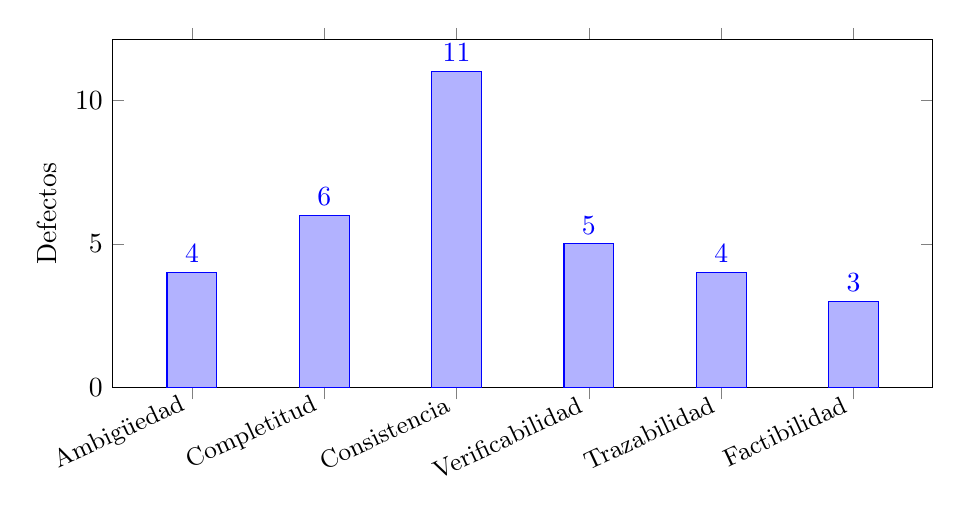
\begin{tikzpicture}
\begin{axis}[
  width=12cm, height=6cm,
  ybar, bar width=18pt,
  ylabel={Defectos},
  symbolic x coords={Ambigüedad,Completitud,Consistencia,Verificabilidad,Trazabilidad,Factibilidad},
  xtick=data, x tick label style={rotate=25,anchor=east,font=\small},
  nodes near coords, ymin=0,
  enlarge x limits=0.12
]
\addplot coordinates {(Ambigüedad,4) (Completitud,6) (Consistencia,11) (Verificabilidad,5) (Trazabilidad,4) (Factibilidad,3)};
\end{axis}
\end{tikzpicture}
\caption{Distribución de defectos por tipo de propiedad evaluada.}
\end{figure}

\begin{figure}[H]
\centering
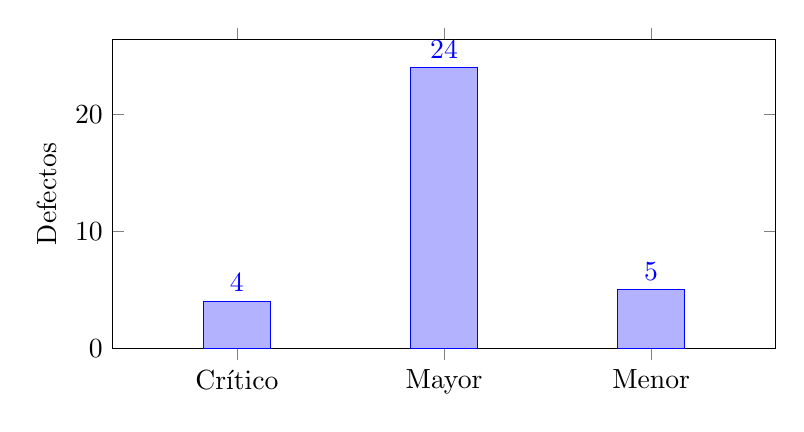
\begin{tikzpicture}
\begin{axis}[
  width=10cm, height=5.5cm,
  ybar, bar width=24pt,
  ylabel={Defectos},
  symbolic x coords={Crítico,Mayor,Menor},
  xtick=data, nodes near coords, ymin=0,
  enlarge x limits=0.3
]
\addplot coordinates {(Crítico,4) (Mayor,24) (Menor,5)};
\end{axis}
\end{tikzpicture}
\caption{Distribución de defectos por severidad asignada.}
\end{figure}

%=======================================================================
% 5. CORRECCIONES
%=======================================================================
\section{Correcciones aplicadas}

Se atendió el cien por ciento de los defectos de severidad crítica y mayor: 28 defectos, de los
cuales 25 se corrigieron directamente sobre las fuentes \LaTeX{} del ERS y 3 se tramitaron ante el
Change Control Board por exceder el alcance de una corrección editorial (véase la \S\ref{sec:ccb}).
Se corrigieron además 4 de los 5 defectos menores, por ser de costo despreciable. El resultado es la
versión \textbf{v1.1} del ERS, cuya línea base se publica con la etiqueta \texttt{baseline-v1.1}.

\noindent\fbox{\parbox{0.96\textwidth}{\small\textbf{Nota sobre la numeración de versiones.} El ERS
del SIMPA registra internamente sus revisiones desde la Entrega 1A y llegó a la Entrega 2A como
revisión interna 3.0. La asignatura, en cambio, designa como \textbf{v1.0} al documento de la
Entrega 2A y como \textbf{v1.1} a la versión resultante de esta práctica. Se adopta la numeración de
la asignatura como versión oficial del documento, y es la única que se declara en la portada del
ERS, en el \id{CHANGELOG.md} y en la etiqueta anotada de Git. Para que la equivalencia sea
verificable y no quede como una discrepancia entre artefactos, el historial del ERS conserva la
columna de revisiones internas y rotula explícitamente la correspondencia
(rev. 3.0 = v1.0, rev. 3.1 = v1.1).}}

\begin{table}[H]
\centering\footnotesize
\caption{Resumen del tratamiento de los defectos}
\begin{tabular}{L{4.6cm} c L{8.5cm}}
\toprule
\textbf{Tratamiento} & \textbf{Defectos} & \textbf{Identificadores}\\
\midrule
Corregidos en el ERS v1.1 & 29 & DEF-01 a DEF-11, DEF-14, DEF-15, DEF-17 a DEF-24, DEF-26 a DEF-33\\
Tramitados ante el CCB & 3 & DEF-12, DEF-13, DEF-16\\
Menores no corregidos & 1 & DEF-25\\
\midrule
\textbf{Total} & \textbf{33} & \\
\bottomrule
\end{tabular}
\end{table}

\subsection*{Defectos derivados al Change Control Board}

Tres defectos no admiten corrección editorial porque su reparación consiste en \emph{añadir alcance}
al sistema, no en enmendar un texto. Corregirlos por decisión unilateral del equipo de análisis
equivaldría a modificar el compromiso de alcance sin gobierno del cambio, que es exactamente lo que
un CCB existe para impedir. Se tramitan por tanto como solicitudes formales, y cada una determina la
naturaleza que la guía exige para las tres RFC:

\begin{itemize}[leftmargin=*, nosep]
  \item \texttt{DEF-13} (crítico) --- \id{RF-36} y \id{RF-37} son \emph{Must} y carecen de historia
        de usuario y de criterio de aceptación. Corregirlo obliga a redactar dos historias nuevas con
        sus escenarios de aceptación. Se tramita como \textbf{RFC-01, de alcance}.
  \item \texttt{DEF-16} (mayor) --- la cobertura declarada de las nueve características de
        ISO/IEC 25010:2023 no se sostiene: ``Portabilidad'' se emplea como característica de primer
        nivel cuando en la edición 2023 es subcaracterística de Flexibilidad, y no existe ningún
        requisito para Seguridad física. Corregirlo obliga a reclasificar \id{RNF-17} y a especificar
        un requisito no funcional nuevo. Se tramita como \textbf{RFC-02, de calidad}.
  \item \texttt{DEF-12} (mayor) --- \id{RL-04}, \id{RL-05} y \id{RL-06} enuncian obligaciones de la
        LOPDP sin ningún requisito funcional que las implemente. Corregirlo obliga a especificar tres
        requisitos funcionales nuevos. Se tramita como \textbf{RFC-03, de restricción normativa}.
\end{itemize}

\noindent
La derivación no relaja la exigencia de corregir el 100\,\% de los críticos y mayores: los tres
quedan cerrados en la misma versión v1.1, con la diferencia de que su incorporación consta en el acta
del CCB y no solo en esta tabla.

\subsection*{Tabla de correcciones}

Cada fila reproduce el texto anterior y el texto resultante en las fuentes \LaTeX{} del ERS. Los
defectos que exigieron más de una edición ---por afectar a varias secciones--- ocupan varias filas
bajo el mismo identificador.

{\footnotesize
\begin{longtable}{p{1.35cm} p{2.1cm} p{5.4cm} p{5.4cm}}
\caption{Correcciones aplicadas al ERS: texto antes y después}\\
\toprule
\textbf{Def.} & \textbf{Req.} & \textbf{Texto antes} & \textbf{Texto después}\\
\midrule
\endfirsthead
\toprule
\textbf{Def.} & \textbf{Req.} & \textbf{Texto antes} & \textbf{Texto después}\\
\midrule
\endhead
\bottomrule
\endfoot
DEF-01 & RD-01 a RD-10 & las nueve características de calidad de ISO/IEC 25010:2023 iso25010, 9 restricciones de & las nueve características de calidad de ISO/IEC 25010:2023 iso25010, 10 restricciones de\\
DEF-02 & Todos los RF & Must (19 RF). Corresponden a tres condiciones. & Must (21 RF). Corresponden a tres condiciones.\\
 &  & (RF-13, RF-14), y el porcentaje de fruta verde determina la penalización del lote en la planta extractora (RF-22, EV-04). & (RF-13, RF-14), y el porcentaje de fruta verde determina la penalización del lote en la planta extractora (RF-22, EV-04). A estas condiciones se añaden RF-36 y RF-37, incorporados a partir de EV-13: [...]\\
 &  & Should (14 RF). Aportan valor sustantivo pero el sistema entrega su propuesta de valor sin ellos en la primera versión: seguimiento de etapas, ficha de plaga, análisis de suelo, recorridos, [...] & Should (16 RF). Aportan valor sustantivo pero el sistema entrega su propuesta de valor sin ellos en la primera versión: seguimiento de etapas, ficha de plaga, análisis de suelo, recorridos, [...]\\
DEF-03 & RF-36 a RF-39 & La tabla completa de clasificación de los 35 requisitos funcionales, con su prioridad MoSCoW, su & La tabla completa de clasificación de los 39 requisitos funcionales, con su prioridad MoSCoW, su\\
DEF-04 & Matriz completa & documento presenta la vista reducida de sus 48 filas y el diagnóstico de cobertura correspondiente. & documento presenta la vista reducida de sus 52 filas y el diagnóstico de cobertura correspondiente.\\
 &  & TR-XX | Fila de la matriz de trazabilidad | TR-01 a TR-48 & TR-XX | Fila de la matriz de trazabilidad | TR-01 a TR-52\\
 &  & Trazabilidad. La matriz enlaza nueve niveles en 48 filas con trece columnas. Se corrigió la & Trazabilidad. La matriz enlaza nueve niveles en 52 filas con trece columnas. Se corrigió la\\
DEF-05 & \S 3.2 completa & Las funciones de alto nivel se agrupan en seis bloques: (i) gestión de la estructura productiva; & Las funciones de alto nivel se agrupan en siete bloques: (i) gestión de la estructura productiva;\\
DEF-06 & RD-01, RD-10, RF-35 & RD-01 | El cliente de campo se ejecuta sobre dispositivos Android 9.0 o superior. | El personal ya dispone de teléfono inteligente propio (EV-05, EV-06, EV-07). & RD-01 | El cliente de campo se ejecuta sobre dispositivos Android 9.0 o superior. | El 88,7\% del personal dispone de teléfono inteligente propio (EV-12), lo que hace de Android la plataforma de mayor [...]\\
DEF-07 & RD-02 & RD-02 | La aplicación opera sin conexión y sincroniza de forma diferida. | La conexión estable se limita al campamento (EV-07); ninguna persona respondiente declaró señal permanente (EV-10). & RD-02 | La aplicación opera sin conexión y sincroniza de forma diferida. | La conexión estable se limita al campamento (EV-07) y el 74,2\% del personal declara no disponer de señal permanente en el [...]\\
DEF-08 & RF-29 & EV-13 | Hoja de liquidación semanal | 03-07/08/2026 | Palmicultora M | RF-29, RF-36 a RF-39 | [P] + [R] | N/A & EV-13 | Hoja de liquidación semanal | 03-07/08/2026 | Palmicultora M | RF-36 a RF-39 | [P] + [R] | N/A\\
DEF-09 & RF-36, RF-37 & RF-35 | Registro delegado del avance | 7,00 | No implementado | - Cobertura verificada del MVP sobre los requisitos funcionales Must & RF-35 | Registro delegado del avance | 7,00 | No implementado | - RF-36 | Catálogo de tarifas por labor | - | No implementado | - RF-37 | Cálculo de la remuneración semanal | - | No implementado | - [...]\\
 &  & Cobertura alcanzada. De los 19 requisitos funcionales Must vigentes al momento de construcción del prototipo, 9 se encuentran implementados de forma completa, 3 de forma parcial y 2 en estado [...] & Cobertura alcanzada. De los 21 requisitos funcionales Must, 8 se encuentran implementados de forma completa, 2 de forma parcial y 2 en estado simulado. La cobertura efectiva es de 8/21 = 38,1\%, o de [...]\\
 &  & computar como implementadas las funcionalidades simuladas, lo que habría permitido reportar un 73,7\% sin sustento verificable. & computar como implementadas las funcionalidades simuladas, lo que habría permitido reportar un 57,1\% sin sustento verificable.\\
 &  & al menos el 60\% de los requisitos Debe tener. El prototipo entregado no alcanza ese umbral. Se declara de forma expresa el valor real (47,4\% completo, 55,3\% ponderado) en lugar de & al menos el 60\% de los requisitos Debe tener. El prototipo entregado no alcanza ese umbral. Se declara de forma expresa el valor real (38,1\% completo, 42,9\% ponderado) en lugar de\\
 &  & Requisitos Must con caso de uso | 19 / 19 (100\%) | Se corrige la deficiencia de la Entrega 2, donde RF-17 y RF-20 carecían de caso de uso. & Requisitos Must con caso de uso | 21 / 21 (100\%) | Se corrige la deficiencia de la Entrega 2, donde RF-17 y RF-20 carecían de caso de uso.\\
 &  & Requisitos Must con historia y criterio | 19 / 19 (100\%) & Requisitos Must con historia y criterio | 19 / 21 (90,5\%) | RF-36 y RF-37 son Must y carecen de historia de usuario y de criterio de aceptación. Su incorporación se tramita mediante RFC-01 ante el [...]\\
 &  & L-10 | El prototipo alcanza una cobertura del 47,4\% de los requisitos Must, por debajo del 60\% exigido por la \S 3.6 de la guía. & L-10 | El prototipo alcanza una cobertura del 38,1\% de los 21 requisitos Must, por debajo del 60\% exigido por la \S 3.6 de la guía.\\
DEF-10 & RF-05, RF-30 & Los cuatro componentes se puntúan en escala Fibonacci (1, 2, 3, 5, 8, 13). La tabla presenta los diez requisitos evaluados de mayor valor de negocio, ordenados de forma descendente por WSJF. & Los cuatro componentes se puntúan en escala Fibonacci (1, 2, 3, 5, 8, 13). La tabla presenta diez de los requisitos evaluados, ordenados de forma descendente por WSJF. No constituye el ranking de los [...]\\
DEF-11 & RF-10 & Lectura del resultado. RF-35 y RF-10 encabezan el orden de implementación con un WSJF de 7,00 cada uno, pese a no ser el requisito de mayor valor de negocio. & Lectura del resultado. RF-35 y RF-10 encabezan el orden de implementación con un WSJF de 7,00 cada uno, pese a no ser los requisitos de mayor valor de negocio. De los dos, solo RF-35 figura en la [...]\\
DEF-14 & RF-36 a RF-39 & Estimación de producción y generación de reportes diarios, semanales y anuales. & Estimación de producción y generación de reportes diarios, semanales y anuales. Ciclo de liquidación semanal: catálogo de tarifas por labor, cálculo de la remuneración a partir del avance registrado, [...]\\
DEF-15 & — & L-06 | Las sesiones de validación walkthrough realizadas son inferiores a las tres exigidas. | Se declara el número efectivo con su acta correspondiente; las restantes se ejecutarán antes de la [...] & L-06 | Las sesiones de validación walkthrough realizadas son inferiores a las tres exigidas: se realizó número efectivo de 3, con acta en 06 Evidencias/. | Las restantes se ejecutarán antes de la [...]\\
DEF-17 & RF-12 & El sistema debe generar alertas ante la detección de plagas, enfermedades, deficiencias nutricionales o condiciones anómalas, dirigidas al rol responsable de su atención. & El sistema debe generar alertas ante cualquiera de los cuatro disparadores siguientes, dirigidas al rol responsable de su atención: (a) diagnóstico positivo de plaga o enfermedad (RF-07); (b) [...]\\
 &  & Pre: existe una incidencia o diagnóstico positivo. Post: la alerta queda registrada con estado abierto hasta su atención. Must Al registrarse un diagnóstico positivo, el sistema genera una alerta [...] & Pre: se cumple al menos uno de los cuatro disparadores enumerados en la descripción. Post: la alerta queda registrada con estado abierto hasta su atención. Must Provocado cada uno de los cuatro [...]\\
DEF-18 & RF-16 & Entrada: registros de avance, recorridos y calificaciones de calidad del período. Salida: indicador de desempeño por persona y período. Pre: existen registros suficientes en el período. Post: el [...] & Entrada: registros de avance, recorridos y calificaciones de calidad del período. Salida: indicador de desempeño por persona y período, expresado en escala de 0 a 100, calculado como el promedio [...]\\
DEF-19 & RF-18 & Pre: existe al menos un censo registrado. Post: la estimación queda disponible para la planificación. Must A partir de un censo y de la variedad del lote, el sistema calcula una estimación de [...] & Pre: existe al menos un censo registrado en los seis meses previos. Post: la estimación queda disponible para la planificación, acompañada de su margen de error declarado. Must Contrastada la [...]\\
DEF-20 & RNF-10 & equivalente a una indisponibilidad <= 7 h 18 min. & equivalente a una indisponibilidad <= 7 h 12 min (720 h x 1\%).\\
DEF-21 & RNF-03 & RNF-03 | Eficiencia de desempeño | Las operaciones de registro y consulta responden en <= 3 s para el percentil 95, con hasta 50 sesiones concurrentes. | Prueba de carga con 50 usuarios virtuales. | [...] & RNF-03 | Eficiencia de desempeño | Las operaciones de registro y consulta responden en <= 3 s para el percentil 95, con hasta 20 sesiones concurrentes. El valor se deriva de la población declarada de [...]\\
DEF-22 & RF-07, RF-08, RF-21 & Pre: la imagen cumple los requisitos mínimos de calidad. Post: el diagnóstico queda asociado al lote y a la fecha. & Pre: la imagen cumple los requisitos mínimos de calidad, que esta ficha define como: resolución no inferior a 1024x768 px, formato JPEG o PNG, tamaño no superior a 5 MB y encuadre en el que el órgano [...]\\
DEF-23 & RF-22 & y emitir una alerta cuando dicho porcentaje se aproxime al umbral a partir del cual la planta extractora aplica penalización. & y emitir una alerta cuando dicho porcentaje alcance el 80\% del umbral a partir del cual la planta extractora aplica penalización. Con el umbral de penalización configurado en el 3\%, la alerta [...]\\
 &  & Configurado un umbral del 3\%, un lote cuya estimación de fruta verde alcance o supere ese valor genera una alerta previa al despacho. & Configurado un umbral de penalización del 3\%, un lote con estimación de fruta verde del 2,4\% o superior genera la alerta preventiva antes del despacho, y un lote con estimación del 2,3\% no la genera.\\
DEF-24 & RF-25, RD-08 & emitiendo una advertencia cuando dicho intervalo supere el valor recomendado para la variedad. & emitiendo una advertencia cuando dicho intervalo supere el valor configurado para la variedad del lote. El valor es un atributo de la variedad, gestionado mediante RF-10, y no una constante del [...]\\
 &  & Pre: existe un registro de cosecha con marca temporal. Post: el intervalo queda registrado junto al despacho. Should Configurado un umbral de 24 horas, un despacho entregado 30 horas después del [...] & Pre: existe un registro de cosecha con marca temporal y la variedad del lote tiene configurado su valor de ventana (RF-10). Post: el intervalo queda registrado junto al despacho. Should Configurado [...]\\
DEF-26 & RF-16, RF-17, RF-20 & Requisitos | RF-19, RF-26 Actores | Primario: administrador general. Precondición | Existen registros en el período seleccionado. & Requisitos | RF-16, RF-17, RF-19, RF-20, RF-26 Actores | Primario: administrador general. Precondición | Existen registros en el período seleccionado.\\
 &  & Flujo alternativo A | Filtrado por lote, por equipo o por persona trabajadora. Flujo alternativo B | Reporte de cumplimiento semanal. & Flujo alternativo A | Filtrado por lote, por equipo o por persona trabajadora. Flujo alternativo C | Reporte de desempeño e historial. El sistema presenta el indicador de desempeño por persona [...]\\
DEF-27 & RF-29, RF-36 a RF-39 & MU-02 | Panel principal | RF-12, RF-19, RF-26 & MU-02 | Panel principal | RF-12, RF-19, RF-26, RF-29, RF-36 a RF-39\\
DEF-28 & — & íntegramente en el archivo referencias.bib. El documento cita 31 fuentes primarias, de las & íntegramente en el archivo referencias.bib. El documento cita 27 fuentes primarias, de las\\
DEF-29 & RF-36 a RF-39 & 3.0 | 03/08/2026 | Equipo AHMRV | Entrega 3 (2A). & 3.0 | 03/08/2026 | Equipo AHMRV | Entrega 3 (2A).\\
 &  & Historial de versiones: la última fila registrada es la 3.0, fechada el 03/08/2026. & Se añade la fila 3.1 con la fecha del acta del CCB, que declara la corrección del 100\% de los defectos críticos y mayores y deja constancia de que la recolección de EV-13 concluyó el 07/08/2026, con posterioridad al cierre de la v3.0.\\
 &  & Versión: 3.0 Fecha: 3 de agosto de 2026 & Versión: 3.1 Fecha: fecha del acta del CCB\\
DEF-30 & RNF-01, RNF-02 & Matriz de confusión sobre conjunto etiquetado independiente de >= 200 imágenes. | EV-04 & Matriz de confusión sobre conjunto etiquetado independiente de >= 200 imágenes. El conjunto no existe (L-05); su construcción se incorpora al alcance de la versión como tarea previa a la [...]\\
 &  & Evaluación sobre conjunto etiquetado por la persona asesora técnica. | EV-01, EV-02 & Evaluación sobre conjunto etiquetado por la persona asesora técnica, sujeta a la misma condición de construcción previa declarada en RNF-01 y en L-05. Hasta entonces, valor objetivo no verificado. | [...]\\
DEF-31 & RF-14, RNF-05 & Pre: sesión iniciada con rastreo GPS activo. Post: el conteo queda registrado sin intervención manual por planta. & Pre: sesión iniciada con rastreo GPS activo. Post: el conteo queda registrado por línea de siembra recorrida, no por planta individual. Nota de alcance: RNF-05 admite una precisión GPS de hasta 10 m. [...]\\
 &  & L-11 | El prototipo carece de servicio de respaldo: & L-12 | No se ha declarado el marco de siembra de la plantación, dato necesario para determinar si la precisión GPS de RNF-05 (<= 10 m) permite discriminar palmas contiguas en RF-14. | RF-14 se acota [...]\\
DEF-32 & — & L-07 | Resuelta. La obtención de la hoja de liquidación semanal (EV-13) incorporó un segundo tipo documental, distinto del plan de labores. | Se dispone de dos tipos documentales de la organización. [...] & L-07 | Resuelta en v3.0; se conserva la fila por trazabilidad histórica y no se contabiliza como limitación vigente. La obtención de la hoja de liquidación semanal (EV-13) incorporó un segundo tipo [...]\\
DEF-33 & RF-15, RF-20 & RF-20 | Historial de actividades y eventos | 2,67 | Implementado | Detalle de lote & (fila eliminada del documento)\\
 &  & RF-15 | Visualización de recorridos del personal | 2,60 | Parcial | Mapa GPS & (fila eliminada del documento)\\
\end{longtable}}

\subsection*{Defectos menores no corregidos}

Un único defecto queda sin corregir: \texttt{DEF-25} (menor). El requisito \id{RF-09} exige recomendar
la acción de control ``según la etapa del insecto'' sin que las etapas del ciclo estén enumeradas ni
acotadas. Corregirlo exige el ciclo biológico de cada una de las plagas del cultivo, información
entomológica que el equipo no posee y que ninguna de las trece evidencias recogidas aporta. Obtenerla
requiere una consulta específica a la persona asesora técnica de la organización, que se programa
antes de la Entrega 4. Se prefiere dejar el requisito declaradamente incompleto antes que enumerar
etapas sin sustento en el dominio: un requisito ambiguo es un defecto conocido, mientras que uno
completado con datos inventados es un defecto oculto.

\subsection*{Valores fijados durante la corrección}

Seis correcciones consistieron en \emph{especificar} un valor que el ERS no declaraba, no en
enmendar uno erróneo. En esos casos el equipo tuvo que elegir la magnitud, y la elección es una
decisión de análisis que debe validarse con la organización antes de la Entrega 4:

\begin{itemize}[leftmargin=*, nosep]
  \item \texttt{DEF-18}: fórmula del indicador de desempeño y pesos de sus tres componentes
        (0,5 / 0,3 / 0,2), declarados configurables.
  \item \texttt{DEF-19}: tolerancia del 20\,\% para la estimación de producción.
  \item \texttt{DEF-21}: 20 sesiones concurrentes, derivadas de la población de 62 personas y del
        25,8\,\% con señal permanente (\id{EV-12}).
  \item \texttt{DEF-22}: umbrales de calidad mínima de la imagen.
  \item \texttt{DEF-23}: disparo de la alerta preventiva al 80\,\% del umbral de penalización.
  \item \texttt{DEF-17}: enumeración cerrada de los cuatro disparadores de alerta.
\end{itemize}

\noindent
Un valor elegido por el equipo es verificable, que es lo que la inspección reclamaba; pero solo es
\emph{correcto} si la organización lo confirma. La distinción se declara aquí para no presentar como
validado lo que por ahora solo está especificado.

%=======================================================================
% 6. CCB
%=======================================================================
\section{Gestión del cambio y Change Control Board}
\label{sec:ccb}

\subsection{Solicitudes formales de cambio}

Se tramitaron tres solicitudes de naturaleza distinta: una de alcance, una de calidad sobre un
requisito no funcional y una de restricción o normativa. Los formularios completos constituyen el
Anexo C y se versionan en \texttt{03\_CCB/}.

Las tres proceden de conflictos reales detectados en la inspección del Paso 1, no de los escenarios
publicados en el SGA. La guía exige que al menos una lo haga; en este caso lo hacen las tres, por una
razón de método: son exactamente los defectos cuya reparación consiste en \emph{añadir alcance} y no
en enmendar un texto, de modo que corregirlos por decisión del equipo de análisis habría equivalido a
modificar el compromiso de alcance sin gobierno del cambio.

\begin{table}[H]
\centering
\caption{Resumen de las solicitudes de cambio tramitadas}
\begin{tabular}{L{1.5cm} L{3cm} L{4.5cm} L{4.5cm}}
\toprule
\textbf{ID} & \textbf{Naturaleza} & \textbf{Origen} & \textbf{Requisito afectado}\\
\midrule
RFC-01 & Alcance & Defecto \texttt{DEF-13} (crítico) de la inspección del Paso 1 & \id{RF-36}, \id{RF-37}\\
RFC-02 & Calidad (RNF) & Defecto \texttt{DEF-16} (mayor) de la inspección del Paso 1 & \id{RNF-17}, \id{RNF-18}\\
RFC-03 & Restricción / normativa & Defecto \texttt{DEF-12} (mayor) de la inspección del Paso 1 & \id{RL-04}, \id{RL-05}, \id{RL-06}\\
\bottomrule
\end{tabular}
\end{table}

\subsection{Análisis de impacto derivado de la matriz de trazabilidad}

El impacto de cada solicitud se obtuvo recorriendo la matriz de trazabilidad
(\texttt{04\_Trazabilidad/matriz\_trazabilidad.xlsx}), filtrando por el requisito afectado y
recogiendo los artefactos enlazados en las columnas hacia adelante. Los identificadores que siguen
son los que devuelve ese filtrado, no una estimación.

{\footnotesize
\begin{longtable}{L{2.4cm} L{4.4cm} L{4.4cm} L{4.4cm}}
\caption{Análisis de impacto de las tres solicitudes de cambio}\\
\toprule
\textbf{Dimensión} & \textbf{RFC-01 (alcance)} & \textbf{RFC-02 (calidad)} & \textbf{RFC-03 (normativa)}\\
\midrule
\endfirsthead
\toprule
\textbf{Dimensión} & \textbf{RFC-01} & \textbf{RFC-02} & \textbf{RFC-03}\\
\midrule
\endhead
\bottomrule
\endfoot
Filas de la matriz & TR-49, TR-50 & TR-46 & TR-03, TR-34 (afectadas); TR-53 a TR-55 (nuevas)\\
Requisitos directos & RF-36, RF-37 & RNF-17, RNF-18 & RL-04, RL-05, RL-06\\
Requisitos indirectos & RF-38, RF-39 (dependen del cálculo de RF-37); RF-28 (fuente del avance que se liquida) & RNF-16 (explicabilidad, misma familia); RF-09 (destinatario del nuevo RNF-19) & RF-03 (gestión de personal), RF-29 (consulta del propio avance), RF-28 (registros a rectificar)\\
Casos de uso & CU-07, CU-08 & CU-18 & CU-08, CU-13\\
Historias de usuario & Ninguna existente: ese es el defecto. Se crean HU-20 y HU-21 & HU-06 & HU-03. Se crean HU-22 a HU-24\\
Prototipos & MU-02 & MU-03 & MU-02\\
Clases y módulos & M-07 Reportes, estimación e histórico & M-05 Diagnóstico asistido por IA & M-01 Gestión de la estructura productiva\\
Casos de prueba & CP-49, CP-50 & CP-41 & CP-03, CP-34; se crean CP-53 a CP-55\\
Efecto sobre RNF & Ninguno. El cálculo opera sobre datos ya registrados & Reclasifica RNF-17 y crea RNF-19; eleva de 18 a 19 los RNF & RNF-12 y RNF-13 (protección de datos) pasan a tener requisitos funcionales que verificarlos\\
Costo estimado & 3 h-persona (redacción de dos historias con escenarios Gherkin y actualización del diagnóstico de cobertura) & 4 h-persona (reclasificación, especificación del RNF de seguridad física y revisión del mapeo a las nueve características) & 14 h-persona (tres fichas de requisito completas, tres historias, tres filas de matriz y actualización de once conteos en cuatro archivos)\\
Riesgo de aprobar & Bajo. No altera el alcance funcional: documenta lo ya especificado & Bajo. RNF-19 condiciona a RF-09, que es \emph{Should} y no está implementado & Medio. Eleva los \emph{Must} de 21 a 24 y reduce la cobertura declarada del MVP del 38,1\,\% al 33,3\,\%\\
Riesgo de rechazar & Alto. Dos requisitos \emph{Must} quedarían sin criterio de aceptación, y la cobertura declarada del 100\,\% sería falsa & Medio. El ERS seguiría declarando una cobertura de las nueve características de ISO/IEC 25010:2023 que no se sostiene & Alto. Tres obligaciones exigibles de la LOPDP quedarían sin requisito que las implemente\\
Alternativas consideradas & Reclasificar RF-36 y RF-37 como \emph{Should}: descartada, porque EV-13 muestra que la liquidación es semanal y central & Declarar la característica no aplicable: descartada, un cultivo con aplicación de agroquímicos tiene riesgo físico real & Diferir a la Entrega 4: descartada en cuanto a la especificación, aceptada en cuanto a la implementación\\
\end{longtable}}

\subsection{Acta del CCB}

\noindent\textbf{Fecha y hora:} {5 de agosto de 2026}, de {08:00} a {09:30}.
\textbf{Modalidad:} sesión presencial en el laboratorio FCCDD-LAB-TIC-201.\\
\textbf{Versión del ERS al abrir la sesión:} v1.0 con las correcciones de la inspección aplicadas.

\begin{table}[H]
\centering\footnotesize
\caption{Asistentes a la sesión del Change Control Board}
\begin{tabular}{L{4.4cm} L{3.4cm} L{7cm}}
\toprule
\textbf{Integrante} & \textbf{Rol en el CCB} & \textbf{Perspectiva que representa}\\
\midrule
Rizzo Vélez Edson Nagib & Presidente & Conduce la deliberación y somete a votación; no vota salvo empate\\
Mora Duarte Alex José & Representante del cliente & Interés de la organización: valor operativo y costo de oportunidad\\
Villafuerte Rosero Allan Noe & Analista y desarrollador & Viabilidad técnica, esfuerzo y efecto sobre los artefactos existentes\\
\bottomrule
\end{tabular}
\end{table}

\noindent
Los cuatro roles del CCB previstos por la guía se cubren con tres personas, por la misma razón
expuesta para el criterio A3 en la \S\ref{sec:inspeccion}: la acumulación de analista y desarrollador
recae sobre un mismo integrante y se declara en lugar de simularse. El presidente se abstiene por
defecto para que la deliberación conserve dos perspectivas efectivamente distintas.

\subsubsection*{Agenda}

\begin{enumerate}[leftmargin=*, nosep]
  \item Verificación del quórum y lectura del análisis de impacto de la \S6.2.
  \item Deliberación y decisión sobre RFC-01, RFC-02 y RFC-03, en ese orden.
  \item Asignación de acciones, responsables y plazos.
  \item Declaración de la versión resultante y autorización de la línea base.
\end{enumerate}

\subsubsection*{Deliberación por solicitud}

\noindent\textbf{RFC-01 --- Historias de usuario y criterios de aceptación de RF-36 y RF-37.}
El representante del cliente sostiene que la liquidación semanal es el proceso que la organización
ejecuta con mayor frecuencia y el que más tiempo administrativo consume, según \id{EV-13}, y que dos
requisitos \emph{Must} sin criterio de aceptación dejan al desarrollo sin condición de cierre
verificable. El analista confirma que el costo es el de redactar dos historias, sin efecto sobre el
alcance funcional, porque el cálculo opera sobre datos que \id{RF-28} ya registra. No se registra
oposición. \textbf{Decisión: aprobado por unanimidad (2 votos a favor, 0 en contra).}

\noindent\textbf{RFC-02 --- Corrección del mapeo a ISO/IEC 25010:2023 y requisito de seguridad
física.} El analista expone que ``Portabilidad'' dejó de ser característica de primer nivel en la
edición 2023 ---sus subcaracterísticas pasaron a Flexibilidad--- y que la novena característica,
Seguridad física, no tiene ningún requisito especificado, de modo que la cobertura declarada de las
nueve no se sostiene. El representante del cliente pregunta si la característica es aplicable a un
sistema de gestión agrícola; el analista responde que sí, porque \id{RF-09} recomienda acciones de
control fitosanitario y una recomendación de agroquímico sin equipo de protección ni intervalo de
reingreso expone físicamente al personal. El representante del cliente retira la objeción y añade
que la asesoría técnica ya exige esos datos en campo. \textbf{Decisión: aprobado por unanimidad
(2 votos a favor, 0 en contra).}

\noindent\textbf{RFC-03 --- Requisitos funcionales para RL-04, RL-05 y RL-06 de la LOPDP.}
El analista advierte que aprobar la solicitud eleva los \emph{Must} de 21 a 24 y reduce la cobertura
declarada del MVP del 38,1\,\% al 33,3\,\%, ya por debajo del umbral exigido. El representante del
cliente responde que el cumplimiento de una obligación legal no es negociable contra una métrica de
avance, y que el riesgo de omitirla recae sobre la organización, no sobre el equipo. El presidente
plantea la alternativa de diferir la especificación a la Entrega 4. El analista objeta que diferirla
dejaría el defecto \texttt{DEF-12} sin cerrar y que el costo de especificar es de 14 horas-persona
frente al de rediseñar más tarde tres funciones que tocan el modelo de datos de personal. Se acuerda
una fórmula intermedia: especificar ahora y construir después.
\textbf{Decisión: aprobado con condiciones (2 votos a favor, 0 en contra).} Condición: los tres
requisitos se incorporan al ERS v1.1 con ficha, historia y criterio completos, y su implementación se
planifica para el incremento de la Entrega 4; la cobertura del MVP se declara con los dos
denominadores.

\subsubsection*{Acciones, responsables y plazos}

\begin{table}[H]
\centering\footnotesize
\caption{Acciones acordadas por el CCB}
\begin{tabular}{L{1.4cm} L{7.2cm} L{3.2cm} L{2.6cm}}
\toprule
\textbf{RFC} & \textbf{Acción} & \textbf{Responsable} & \textbf{Plazo}\\
\midrule
RFC-01 & Redactar HU-20 y HU-21 con escenarios Gherkin y actualizar el diagnóstico de cobertura de la \S5.4.1 & Mora Duarte & {07/08/2026}\\
RFC-02 & Reclasificar RNF-17 bajo Flexibilidad, especificar RNF-19 y revisar el mapeo de las nueve características & Villafuerte Rosero & {08/08/2026}\\
RFC-03 & Especificar RF-40 a RF-42, redactar HU-22 a HU-24, añadir TR-53 a TR-55 y actualizar los conteos afectados & Villafuerte Rosero & {09/08/2026}\\
RFC-03 & Planificar la implementación de RF-40 a RF-42 en el incremento de la Entrega 4 & Rizzo Vélez & Entrega 4\\
--- & Publicar el ERS v1.1 y la etiqueta \texttt{baseline-v1.1} & Rizzo Vélez & {10/08/2026}\\
\bottomrule
\end{tabular}
\end{table}

\subsubsection*{Cierre}

Aprobadas las tres solicitudes, el CCB autoriza la publicación del ERS en su versión \textbf{v1.1} y
el establecimiento de la línea base correspondiente. Se levanta la sesión.

\vspace{0.8cm}
\noindent\begin{tabular}{p{4.7cm} p{4.7cm} p{4.7cm}}
\hrulefill & \hrulefill & \hrulefill\\
\footnotesize Rizzo Vélez Edson Nagib & \footnotesize Mora Duarte Alex José & \footnotesize Villafuerte Rosero Allan Noe\\
\footnotesize Presidente del CCB & \footnotesize Representante del cliente & \footnotesize Analista y desarrollador\\
\end{tabular}

\subsection{Versión resultante del ERS}

La aplicación de los cambios aprobados eleva el ERS de la versión v1.0 a la versión v1.1. La versión
declarada es idéntica en la portada del ERS, en su historial de revisiones, en el archivo
\texttt{CHANGELOG.md} y en la etiqueta anotada de Git.

\begin{table}[H]
\centering\footnotesize
\caption{Efecto acumulado de las tres solicitudes sobre el ERS}
\begin{tabular}{L{6cm} c c L{4.6cm}}
\toprule
\textbf{Magnitud} & \textbf{v1.0} & \textbf{v1.1} & \textbf{Origen del cambio}\\
\midrule
Requisitos funcionales & 39 & 42 & RFC-03\\
Requisitos no funcionales & 18 & 19 & RFC-02\\
Requisitos funcionales \emph{Must} & 21 & 24 & RFC-03\\
Historias de usuario & 19 & 24 & RFC-01 y RFC-03\\
Filas de la matriz de trazabilidad & 52 & 55 & RFC-03\\
\emph{Must} con historia y criterio & 19 / 21 & 24 / 24 & RFC-01 y RFC-03\\
Cobertura del MVP sobre \emph{Must} & 38,1\,\% & 33,3\,\% & RFC-03 (denominador mayor)\\
Páginas del documento & 80 & 87 & Acumulado\\
\bottomrule
\end{tabular}
\end{table}

\noindent
La última fila de cobertura merece una lectura explícita: el CCB aprobó un conjunto de cambios que
\emph{empeora} la métrica de cobertura del prototipo. Un órgano de control de cambios que solo
aprobara lo que mejora sus propios indicadores no estaría gobernando el alcance, sino administrando
la apariencia del proyecto. La cobertura se declara con los dos denominadores ---38,1\,\% sobre el
alcance vigente cuando se construyó el prototipo y 33,3\,\% sobre el alcance posterior al CCB---
porque responden a preguntas distintas y ninguna sustituye a la otra.

%=======================================================================
% 7. TRAZABILIDAD EN JIRA
%=======================================================================
\section{Trazabilidad en herramienta CASE}
\label{sec:trazabilidad}

\subsection{Estructura del tablero}

El proyecto se creó en Jira con el nombre del sistema del PFC y acceso para los integrantes y el
docente. Se optó por un proyecto \emph{company-managed} y no \emph{team-managed}: la documentación
de Atlassian establece que los campos personalizados de un proyecto \emph{team-managed} quedan
contenidos en ese proyecto y no pueden compartirse ni reutilizarse, mientras que los de un proyecto
\emph{company-managed} son administrables globalmente \cite{atlassianfields}. Dado que la práctica
exige campos personalizados poblados y visibles en la vista de incidencia, la segunda modalidad es
la única que garantiza el resultado.

La carga inicial del backlog se realizó por importación CSV. El archivo de importación
(\texttt{04\_Trazabilidad/backlog\_import\_jira.csv}) se construyó extrayendo campo por campo las 39
fichas de requisito de la \S3.2 del ERS, de modo que ningún elemento del tablero carece de
correspondencia en el documento fuente. Es un archivo distinto del Anexo D, que es la exportación
que produce Jira una vez creado el tablero.

\begin{table}[H]
\centering
\caption{Estructura del backlog en Jira}
\begin{tabular}{L{3.5cm} L{3cm} L{6.5cm}}
\toprule
\textbf{Nivel} & \textbf{Cantidad} & \textbf{Criterio de organización}\\
\midrule
Epics & 7 & Una épica por bloque funcional de la \S3.2 del ERS (Bloque~I a Bloque~VII)\\
Stories & 39 & Una historia por requisito funcional, de \texttt{RF-01} a \texttt{RF-39}\\
Sub-tasks & 38, en 19 historias & Dos por historia: el criterio de aceptación en formato Gherkin de la \S5.2 y el criterio de verificación de la ficha de la \S3.2\\
\bottomrule
\end{tabular}
\end{table}

\subsection{Campos personalizados}

\begin{table}[H]
\centering
\caption{Campos personalizados configurados}
\begin{tabular}{L{4cm} L{3.5cm} L{7cm}}
\toprule
\textbf{Campo} & \textbf{Tipo} & \textbf{Valores}\\
\midrule
Prioridad MoSCoW & Lista desplegable & Must / Should / Could / Won't. El valor se toma de la ficha del requisito en la \S3.2 del ERS y no de la \S5.3.1, porque ambas se contradicen (defecto \texttt{DEF-02}) y solo las fichas admiten conteo directo\\
Fuente del requisito & Texto multilínea & Parte interesada de origen e identificadores de evidencia de campo (\texttt{EV-01} a \texttt{EV-13}), transcritos del campo ``Actor / Origen'' de la ficha del requisito\\
Estado de verificación & Lista desplegable & Pendiente de verificación / En verificación / Verificado / No verificable en v1\\
\bottomrule
\end{tabular}
\end{table}

\subsection{Matriz de trazabilidad}

La matriz completa, con sus trece columnas y la declaración de procedencia de cada una, reside en
\texttt{04\_Trazabilidad/matriz\_trazabilidad.xlsx}. La vista siguiente reproduce sus 52 filas en el
formato exigido por la guía. Las columnas de interesado y requisito se transcriben de la Tabla~69
del ERS; las de módulo y prueba son derivadas por el equipo, porque el ERS no especifica ni módulos
de implementación ni casos de prueba: el módulo corresponde al bloque funcional de la \S3.2 en que
el propio ERS ubica cada requisito, y el caso de prueba se deriva del campo ``criterio de
verificación'' de la ficha, que es la única condición de aceptación enunciada por requisito.

\begin{longtable}{p{2.6cm} p{1.4cm} p{1.4cm} p{5.4cm} p{1.8cm}}
\caption{Matriz de trazabilidad bidireccional (52 filas)}\\
\toprule
\textbf{Stakeholder} & \textbf{RF} & \textbf{CU} & \textbf{Clase / Módulo} & \textbf{Prueba}\\
\midrule
\endfirsthead
\toprule
\textbf{Stakeholder} & \textbf{RF} & \textbf{CU} & \textbf{Clase / Módulo} & \textbf{Prueba}\\
\midrule
\endhead
\bottomrule
\endfoot
Administrador & RF-01 & CU-11 & M-01 Gestión de la estructura productiva & CP-01\\
Administrador & RF-02 & CU-12 & M-01 Gestión de la estructura productiva & CP-02\\
Administrador & RF-03 & CU-13 & M-01 Gestión de la estructura productiva & CP-03\\
Trabajador & RF-04 & CU-04 & M-03 Registro operativo de campo & CP-04\\
Trabajador & RF-04 & CU-04 & M-03 Registro operativo de campo & CP-04\\
Técnico fitosan. & RF-05 & CU-15 & M-03 Registro operativo de campo & CP-05\\
Administrador & RF-06 & CU-12 & M-03 Registro operativo de campo & CP-06\\
Asistente admin. & RF-07 & CU-01 & M-05 Diagnóstico asistido por IA & CP-07\\
Asistente admin. & RF-07 & CU-01 & M-05 Diagnóstico asistido por IA & CP-07\\
Asesor técnico & RF-08 & CU-02 & M-05 Diagnóstico asistido por IA & CP-08\\
Asesor técnico & RF-08 & CU-02 & M-05 Diagnóstico asistido por IA & CP-08\\
Técnico fitosan. & RF-09 & CU-01 & M-05 Diagnóstico asistido por IA & CP-09\\
Asesor técnico & RF-10 & CU-12 & M-01 Gestión de la estructura productiva & CP-10\\
Asesor técnico & RF-11 & CU-02 & M-03 Registro operativo de campo & CP-11\\
Administrador & RF-12 & CU-16 & M-05 Diagnóstico asistido por IA & CP-12\\
Trabajador & RF-12 & CU-16 & M-05 Diagnóstico asistido por IA & CP-12\\
Jefe polinización & RF-13 & CU-03 & M-04 Polinización asistida & CP-13\\
Jefe polinización & RF-14 & CU-03 & M-04 Polinización asistida & CP-14\\
Administrador & RF-15 & CU-03 & M-04 Polinización asistida & CP-15\\
Administrador & RF-16 & CU-05 & M-04 Polinización asistida & CP-16\\
Administrador & RF-17 & CU-05 & M-03 Registro operativo de campo & CP-17\\
Administrador & RF-18 & CU-17 & M-07 Reportes, estimación e histórico & CP-18\\
Administrador & RF-19 & CU-05 & M-07 Reportes, estimación e histórico & CP-19\\
Administrador & RF-20 & CU-05 & M-07 Reportes, estimación e histórico & CP-20\\
Téc. extractora & RF-21 & CU-06 & M-05 Diagnóstico asistido por IA & CP-21\\
Téc. extractora & RF-21 & CU-06 & M-05 Diagnóstico asistido por IA & CP-21\\
Administrador & RF-22 & CU-06 & M-06 Calidad de la fruta y relación con la extractora & CP-22\\
Administrador & RF-23 & CU-10 & M-06 Calidad de la fruta y relación con la extractora & CP-23\\
Téc. extractora & RF-24 & CU-10 & M-06 Calidad de la fruta y relación con la extractora & CP-24\\
Téc. extractora & RF-25 & CU-10 & M-06 Calidad de la fruta y relación con la extractora & CP-25\\
Administrador & RF-26 & CU-07 & M-02 Planificación y seguimiento de labores & CP-26\\
Administrador & RF-27 & CU-07 & M-02 Planificación y seguimiento de labores & CP-27\\
Trabajador & RF-28 & CU-04 & M-03 Registro operativo de campo & CP-28\\
Trabajador & RF-29 & CU-08 & M-03 Registro operativo de campo & CP-29\\
Asistente admin. & RF-30 & CU-09 & M-03 Registro operativo de campo & CP-30\\
Asistente admin. & RF-31 & CU-09 & M-03 Registro operativo de campo & CP-31\\
Téc. extractora & RF-32 & CU-17 & M-07 Reportes, estimación e histórico & CP-32\\
Téc. extractora & RF-33 & CU-10 & M-06 Calidad de la fruta y relación con la extractora & CP-33\\
Administrador & RF-34 & CU-07 & M-02 Planificación y seguimiento de labores & CP-34\\
Jefe de campo & RF-35 & CU-04 & M-02 Planificación y seguimiento de labores & CP-35\\
Téc. extractora & RNF-01 & CU-06 & M-05 Diagnóstico asistido por IA (vía CU) & CP-36\\
Trabajador & RNF-11 & CU-04 & M-03 Registro operativo de campo (vía CU) & CP-37\\
Jefe polinización & RNF-05 & CU-03 & M-04 Polinización asistida (vía CU) & CP-38\\
Trabajador & RNF-08 & CU-04 & M-03 Registro operativo de campo (vía CU) & CP-39\\
Trabajador & RNF-14 & CU-03 & M-04 Polinización asistida (vía CU) & CP-40\\
Asistente admin. & RNF-16 & CU-18 & M-05 Diagnóstico asistido por IA (vía CU) & CP-41\\
Trabajador & RD-10 & CU-04 & M-03 Registro operativo de campo (vía CU) & CP-42\\
Téc. extractora & RD-07 & CU-06 & M-05 Diagnóstico asistido por IA (vía CU) & CP-43\\
Administrador & RF-36 & CU-08 & M-02 Planificación y seguimiento de labores & CP-44\\
Administrador & RF-37 & CU-07 & M-02 Planificación y seguimiento de labores & CP-45\\
Administrador & RF-38 & CU-07 & M-02 Planificación y seguimiento de labores & CP-46\\
Administrador & RF-39 & CU-07 & M-02 Planificación y seguimiento de labores & CP-47\\
\end{longtable}

\subsection*{Requisitos huérfanos}

La matriz cierra hacia atrás en las 52 filas: los 39 requisitos funcionales tienen parte interesada
y evidencia de origen identificadas, sin excepción. Hacia adelante se detectan tres vacíos, que se
reportan de forma explícita:

\begin{enumerate}[leftmargin=*, nosep]
  \item \textbf{Requisitos sin prototipo de interfaz.} \texttt{RF-03}, \texttt{RF-27} y
        \texttt{RF-34}. Los tres son de prioridad distinta de \emph{Must}, por lo que el vacío no
        incumple la exigencia de prototipar las pantallas \emph{Must}. Se localizan en el tablero
        con el filtro \texttt{labels = "MU:sin-mockup"}.
  \item \textbf{Requisitos \emph{Must} sin historia de usuario ni criterio de aceptación.}
        \texttt{RF-36} y \texttt{RF-37}. Es el mismo hallazgo que el defecto \texttt{DEF-13} de la
        inspección, y el tablero lo hace visible sin necesidad de releer el ERS: son las dos únicas
        historias de prioridad \emph{Must} que no despliegan sub-tareas. Contradice la Tabla~70 del
        ERS, que declara una cobertura de 19/19 (100\,\%) de los \emph{Must} con historia y
        criterio.
  \item \textbf{Requisitos con fuente única.} \texttt{RF-11}, \texttt{RF-23}, \texttt{RF-25},
        \texttt{RF-32}, \texttt{RF-33} y \texttt{RF-34} se sustentan en una sola evidencia. El ERS
        ya declara esta limitación en su \S5.4; la inspección la confirma y no la agrega como
        defecto nuevo, porque un vacío declarado no es un defecto oculto.
\end{enumerate}

\noindent
El conteo de las 39 fichas de la \S3.2 arroja 21 requisitos \emph{Must}, 16 \emph{Should} y 2
\emph{Could}. Este resultado, obtenido al poblar el tablero, resuelve en una dirección concreta la
contradicción del defecto \texttt{DEF-02}: la cifra correcta es la de la \S5.1 del ERS y la
errónea la de la \S5.3.1. La trazabilidad, construida como instrumento de gestión, terminó
funcionando como instrumento de validación.

\subsection*{Evidencias}

Las capturas del tablero completo, del detalle de al menos tres incidencias con sus enlaces visibles
y del panel de estadísticas se incluyen en el Anexo E. La exportación del backlog en formato CSV
constituye el Anexo D y reside en \texttt{04\_Trazabilidad/backlog\_export.csv}.

%=======================================================================
% 8. LINEA BASE CON GIT
%=======================================================================
\section{Línea base con Git}

\subsection{Repositorio}

El repositorio público del equipo se encuentra en\\
\url{https://github.com/erizzov-boop/ISR401-PFC-ERS-EQUIPO_B}\\
 Su archivo \texttt{README.md} documenta el
sistema, los integrantes, la estructura de carpetas y las instrucciones de compilación del presente
informe.

\subsection{Commits semánticos y autoría}

\begin{table}[H]
\centering
\caption{Distribución de commits por integrante}
\begin{tabular}{L{5cm} c L{6.5cm}}
\toprule
\textbf{Integrante} & \textbf{Commits} & \textbf{Artefactos aportados}\\
\midrule
Mora Duarte Alex José & \pendiente{} & \pendiente{}\\
Rizzo Vélez Edson Nagib & \pendiente{} & \pendiente{}\\
Villafuerte Rosero Allan Noe & \pendiente{} & \pendiente{}\\
\midrule
\textbf{Total} & \pendiente{$\geq 8$} & \\
\bottomrule
\end{tabular}
\end{table}

\subsection{Etiqueta anotada de línea base}

\begin{lstlisting}[basicstyle=\footnotesize\ttfamily, frame=single]
git tag -a baseline-v1.1 -m "Baseline aprobada por CCB"
git push origin baseline-v1.1
\end{lstlisting}

\subsection{Registro de cambios}

El archivo \texttt{CHANGELOG.md} sigue el formato \emph{[Versión] --- [Fecha] / Añadido / Cambiado /
Eliminado} e incorpora una entrada por cada RFC aprobado, identificada con su código.

\subsection{Historial}

Las capturas de \texttt{git log --oneline --graph --decorate} y de \texttt{git tag -n} se incluyen en
el Anexo E.

%=======================================================================
% 9. COMPARATIVA CASE
%=======================================================================
\section{Comparativa de herramientas CASE}
\label{sec:comparativa}

Los seis criterios se toman del conjunto de funcionalidades esperables en una herramienta de
gestión de requisitos --- repositorio, atributos, trazabilidad, \emph{baselining}, control de
cambios, colaboración e integración con el control de versiones --- que Wiegers y Beatty
\cite{wiegers2013} y Pohl \cite{pohl2025} identifican como el núcleo de la categoría. El juicio de
cada celda para Jira procede de su uso efectivo durante esta práctica; el de las otras tres, de su
documentación oficial de producto. Se hace explícito qué se verificó y qué no: el equipo no operó
DOORS Next, Jama Connect ni ReqView, y por tanto no emite juicio de uso sobre ellas.

{\scriptsize
\begin{longtable}{L{1.9cm} L{2.5cm} L{2.5cm} L{2.5cm} L{2.5cm} L{1.5cm}}
\caption{Comparativa de herramientas CASE para gestión de requisitos}\\
\toprule
\textbf{Criterio} & \textbf{Jira} & \textbf{IBM DOORS Next} & \textbf{Jama Connect} & \textbf{ReqView} & \textbf{Fuente}\\
\midrule
\endfirsthead
\toprule
\textbf{Criterio} & \textbf{Jira} & \textbf{IBM DOORS Next} & \textbf{Jama Connect} & \textbf{ReqView} & \textbf{Fuente}\\
\midrule
\endhead
\bottomrule
\endfoot
Funcionalidades de IR
& No es una herramienta de IR: es un gestor de incidencias al que hay que \emph{construirle} la semántica de requisito con campos personalizados. Los tres campos de esta práctica hubo que crearlos y asociarlos a pantallas manualmente.
& Herramienta de IR nativa: módulos de especificación estructurada, atributos tipados, líneas base y firma electrónica forman parte del producto, no de una configuración.
& Nativa y orientada a producto regulado; incorpora revisiones formales, gestión de riesgo y cobertura de verificación como objetos de primer orden.
& Nativa y deliberadamente mínima: requisitos, riesgos y pruebas como tipos de objeto, con atributos personalizables y sin capa de proceso impuesta.
& Uso propio (PE4); \cite{ibmdoorsnext,jamatrace,reqview}\\
\midrule
Trazabilidad
& Solo la que el equipo construya: jerarquía épica--historia--sub-tarea, más enlaces y etiquetas. La matriz de 52 filas se mantuvo fuera de Jira, en hoja de cálculo, porque el tablero no genera vistas de trazabilidad multinivel.
& Trazabilidad multinivel con vistas configurables y análisis de impacto sobre el propio repositorio.
& Trazabilidad ``viva'' entre elementos con reglas de relación que imponen el modelo de la organización, y métricas de cobertura calculadas por la herramienta.
& Matriz de trazabilidad e informes multinivel exportables a Word, Excel, PDF y HTML.
& Uso propio (PE4); \cite{ibmdoorsnext,jamatrace,reqview}\\
\midrule
Colaboración
& Fuerte y de bajo umbral: comentarios, menciones, tableros compartidos. Fue el criterio que más pesó para un equipo de tres personas sin experiencia previa en herramientas de IR.
& Colaboración sobre plataforma Jazz con paneles, revisiones y comentarios; administración centralizada de usuarios y tipos.
& Revisiones formales con registro de aprobaciones y versiones, pensadas para dejar evidencia auditable de la validación.
& Colaboración indirecta: el proyecto es un archivo versionado, de modo que la concurrencia se resuelve con el flujo de trabajo de Git y no dentro de la herramienta.
& Uso propio (PE4); \cite{ibmdoorsnext,jamatrace,reqview}\\
\midrule
Integración con VCS
& Indirecta: se logra por convención en los mensajes de \emph{commit} y por vinculación de ramas y \emph{pull requests} a la incidencia \cite{clelandhuang2012}. En esta práctica el vínculo entre el tablero y el repositorio es una convención del equipo, no una función de la herramienta.
& Integración por la vía del ecosistema de ingeniería del proveedor más que por acoplamiento directo a un VCS de propósito general.
& Integración con Jira y con entornos de desarrollo para mantener la trazabilidad entre requisito y trabajo de desarrollo.
& El proyecto se almacena en Git o Subversion de forma nativa: el requisito es un objeto versionado con el mismo mecanismo que el código.
& Uso propio (PE4); \cite{clelandhuang2012,ibmdoorsnext,jamatrace,reqview}\\
\midrule
Costo
& Plan gratuito suficiente para un equipo de tres personas; fue el factor decisivo dada la restricción presupuestaria de una práctica académica.
& Licenciamiento empresarial, dimensionado para programas de ingeniería de sistemas de larga duración; fuera del alcance de un PFC.
& Licenciamiento empresarial orientado a industria regulada.
& Suscripción anual por usuario con versión gratuita limitada; la más accesible de las tres herramientas de IR nativas.
& \cite{reqview}; documentación de producto\\
\midrule
Curva de aprendizaje
& Baja para el uso básico y alta para el uso como herramienta de IR: la dificultad no está en aprender Jira sino en decidir cómo representar un requisito dentro de él, decisión que la herramienta no guía.
& Alta: exige comprender el modelo de artefactos, tipos y configuraciones de la plataforma antes de producir valor.
& Media-alta: el modelo conceptual es más cercano al vocabulario de la IR, pero la configuración de reglas de relación exige decisiones de método previas.
& Baja: el modelo tabular es próximo a la hoja de cálculo que el equipo ya venía usando para la matriz.
& Uso propio (PE4); \cite{ibmdoorsnext,jamatrace,reqview}\\
\end{longtable}}

\subsection*{Recomendación para el PFC}

Para el SIMPA se recomienda \textbf{mantener Jira} en el corto plazo y \textbf{migrar la matriz a ReqView} si
el proyecto continúa más allá del PFC. La recomendación no se apoya en que Jira sea la mejor
herramienta de gestión de requisitos --- no lo es, y esta práctica lo mostró de forma directa: los
39 requisitos entraron al tablero, pero la matriz de 52 filas tuvo que mantenerse fuera de él, en
hoja de cálculo, porque Jira no produce vistas de trazabilidad multinivel. Se apoya en tres
condiciones concretas del proyecto. Primera, el costo: el plan gratuito cubre a los tres
integrantes, y ninguna de las tres alternativas nativas tiene un equivalente utilizable sin
licencia. Segunda, la curva de aprendizaje frente al plazo: la práctica dispone de 1,5~horas para
el bloque de trazabilidad, y en ese tiempo el equipo pudo crear el proyecto, configurar tres campos
personalizados e importar 84 elementos. Tercera, la naturaleza del SIMPA: es un sistema de gestión
agrícola sin exigencia de certificación, de modo que las capacidades por las que se paga DOORS Next
o Jama Connect --- firma electrónica, cobertura de verificación auditable, cumplimiento normativo
sectorial --- no corresponden al problema.

La recomendación de ReqView para una eventual continuación se sustenta en el criterio que más pesó
en la inspección: el ERS del SIMPA falló principalmente por consistencia entre secciones, no por
falta de contenido. ReqView versiona el proyecto directamente en Git \cite{reqview}, lo que
permitiría que el ERS y su matriz evolucionen bajo el mismo mecanismo de línea base que el equipo ya
estableció en esta práctica, en lugar de mantener dos historiales paralelos --- el del documento y
el del tablero --- que es exactamente la situación que produjo los once defectos de consistencia
detectados.

%=======================================================================
% 10. TRADICIONAL VS AGIL
%=======================================================================
\section{Ingeniería de requisitos tradicional frente a ágil}

\begin{table}[H]
\centering\footnotesize
\caption{Contraste entre el enfoque documental y el enfoque ágil}
\begin{tabular}{L{2.6cm} L{4.7cm} L{4.7cm} L{2.3cm}}
\toprule
\textbf{Dimensión} & \textbf{IR tradicional} & \textbf{IR ágil} & \textbf{Contexto favorable}\\
\midrule
Documentación
& El ERS es el artefacto contractual: completo antes de construir, con estructura normalizada por ISO/IEC/IEEE 29148 \cite{iso29148}.
& La documentación es el \emph{backlog}: historias con criterios de aceptación que se detallan justo antes de implementarse \cite{cohn2004}.
& Tradicional cuando el requisito debe ser auditable o contractual\\
Gestión del cambio
& Cambio controlado: RFC, análisis de impacto sobre la matriz y decisión de un CCB \cite{pmbok7}.
& Cambio esperado: reordenar el \emph{backlog} es una operación ordinaria, no un evento de gobierno.
& Tradicional con dependencias fuertes; ágil con requisitos volátiles\\
Participación de stakeholders
& Concentrada en la elicitación y en hitos de validación; entre hitos, el documento sustituye a la persona.
& Continua, con retroalimentación por incremento y refinamiento periódico del \emph{backlog} \cite{ireb31}.
& Ágil cuando el interesado está disponible; tradicional cuando no lo está\\
Herramientas
& Herramientas de IR con repositorio, atributos, líneas base y trazabilidad multinivel.
& Gestores de \emph{backlog} y de incidencias, con la trazabilidad reconstruida por convención sobre ramas y \emph{commits} \cite{clelandhuang2012}.
& Tradicional si la trazabilidad debe demostrarse; ágil si basta con mantenerla\\
Velocidad
& Lenta al inicio y estable después: el costo se paga antes de construir.
& Rápida al inicio: se entrega valor antes de haber especificado el conjunto.
& Ágil con incertidumbre alta de mercado; tradicional con costo alto de error\\
Escalabilidad
& Escala en número de requisitos y de organizaciones: la especificación es el mecanismo de coordinación.
& Escala en número de iteraciones, no de interlocutores; con muchos equipos exige marcos adicionales de coordinación \cite{swebok4}.
& Tradicional en sistemas de sistemas; ágil en producto único con un equipo\\
\bottomrule
\end{tabular}
\end{table}

El SIMPA no se sitúa limpiamente en ninguno de los dos extremos, y esta práctica lo evidenció. El
proyecto produjo un ERS documental completo --- 39 requisitos funcionales, 18 no funcionales, 10
restricciones y 8 requisitos legales --- y al mismo tiempo mantiene 19 historias de usuario con
criterios de aceptación en formato Gherkin \cite{smart2014}. Los dos artefactos conviven, y la
inspección mostró el costo de esa convivencia: cuatro de los once defectos de consistencia nacen
justamente de que las mismas cifras se declaran de forma distinta en la parte documental y en la
parte de priorización del documento. La conclusión práctica no es que uno de los dos enfoques
sobrara, sino que mantener ambos exige un mecanismo de reconciliación que el ERS no tenía.

El contexto del SIMPA inclina la balanza hacia el enfoque documental en un punto concreto y hacia
el ágil en otro. Hacia el documental, por la LOPDP: los ocho requisitos legales del ERS deben poder
demostrarse ante un tercero, y una obligación legal no se satisface con una historia de usuario
priorizada. Hacia el ágil, por la volatilidad efectiva del dominio: la evidencia \texttt{EV-13},
recogida después de cerrada la especificación, obligó a añadir cuatro requisitos nuevos
(\texttt{RF-36} a \texttt{RF-39}) sobre un proceso --- la liquidación semanal --- que el equipo no
había identificado en las doce evidencias anteriores. Un ERS cerrado no absorbe ese hallazgo sin
una entrada de cambio formal, que es precisamente lo que el CCB de esta práctica tramita.

%=======================================================================
% 11. CONCLUSIONES
%=======================================================================
\section{Conclusiones críticas}


\begin{enumerate}[leftmargin=*]
  \item {Validación: La inspección Fagan reveló que el ERS del SIMPA no falla por errores puntuales de redacción, sino por falta de reconciliación entre secciones: con una densidad de 0,52 defectos por página y 11 de los 33 defectos clasificados como "consistencia" (un tercio del total, DEF-01 a DEF-11), la causa raíz no es la calidad de cada enunciado individual sino la ausencia de una pasada final que unifique cifras repetidas en distintas tablas (por ejemplo, la distribución MoSCoW declarada dos veces de forma contradictoria en DEF-02). Esto confirma empíricamente, con datos del propio equipo, que un documento "crecido por adición" necesita inspección formal periódica, no solo al cierre.}
  \item {Gestión del cambio: La deliberación de RFC-03 en el CCB mostró que gobernar el cambio no es optimizar métricas: el comité aprobó una solicitud que empeoró la cobertura declarada del MVP del 38,1 al 33,3 (al elevar los requisitos Must de 21 a 24), porque el cumplimiento de las obligaciones legales de la LOPDP (RL-04 a RL-06) no podía subordinarse a un indicador de avance. La condición pactada —especificar ahora, implementar en la Entrega 4— evidenció que un CCB funcional separa la decisión de alcance de la decisión de calendario, algo que una corrección editorial unilateral del equipo de análisis nunca podría haber resuelto con la misma trazabilidad de responsabilidad.}
  \item {Trazabilidad: La matriz de trazabilidad, aunque completa en 52 filas, expuso fallas de cierre bidireccional que solo aparecen al recorrerla en ambos sentidos: DEF-26 mostró que la matriz vincula RF-16, RF-17 y RF-20 al caso de uso CU-05, mientras que la especificación textual de CU-05 solo reconoce RF-19 y RF-26; DEF-27 encontró una discrepancia equivalente entre la matriz y el prototipo MU-02. Esto demuestra que una matriz puede estar "completa" en número de filas y aun así no ser trazable en la práctica, porque la trazabilidad bidireccional exige verificar la consistencia entre el artefacto derivado y su fuente, no solo la existencia del enlace.}
  \item {Herramientas: La experiencia con Jira confirmó que una herramienta de gestión de incidencias no sustituye a una herramienta de IR nativa: el equipo tuvo que construir manualmente la semántica de requisito (los tres campos personalizados) y, pese a ello, la matriz de 52 filas debió mantenerse fuera del tablero, en hoja de cálculo, porque Jira no genera vistas de trazabilidad multinivel. La recomendación resultante —mantener Jira por costo y curva de aprendizaje en el corto plazo, pero migrar a ReqView si el SIMPA continúa— no es una preferencia abstracta, sino la respuesta directa al hallazgo del punto 1: ReqView versiona el proyecto en Git, lo que eliminaría el doble historial (documento vs. tablero) que produjo los once defectos de consistencia.}
  \item {Integración de los cuatro temas: El caso RFC-03 conecta los cuatro ejes de la unidad en una sola cadena de causalidad: un defecto de completitud detectado en la inspección (DEF-12, obligaciones LOPDP sin requisito funcional) se tramitó como solicitud formal de cambio ante el CCB, cuya aprobación modificó la matriz de trazabilidad (de 52 a 55 filas) y quedó registrada mediante control de versiones (línea base v1.1, etiqueta baseline-v1.1). Ninguna de las cuatro prácticas —validar, gestionar el cambio, trazar y versionar— habría sido suficiente por sí sola: sin la inspección el defecto no se habría detectado; sin el CCB se habría corregido sin gobierno del alcance; sin la matriz actualizada la corrección no sería verificable; y sin la línea base no habría evidencia auditable de cuándo y por qué cambió el ERS.}
\end{enumerate}

%=======================================================================
% 12. DISTRIBUCION DEL TRABAJO
%=======================================================================
\section{Distribución del trabajo}

\begin{table}[H]
\centering
\caption{Aportes por integrante, contrastables con el historial de commits}
\begin{tabular}{L{4.5cm} L{7cm} c}
\toprule
\textbf{Integrante} & \textbf{Aporte principal} & \textbf{Commits}\\
\midrule
Mora Duarte Alex José & \pendiente{} & \pendiente{}\\
Rizzo Vélez Edson Nagib & \pendiente{} & \pendiente{}\\
Villafuerte Rosero Allan Noe & \pendiente{} & \pendiente{}\\
\bottomrule
\end{tabular}
\end{table}

%=======================================================================
% 13. REFERENCIAS
%=======================================================================
\newpage
% Si falta IEEEtran.bst (paquete texlive-publishers) se degrada a unsrt
% en lugar de abortar la compilacion. Para la entrega debe estar IEEEtran.
\IfFileExists{IEEEtran.bst}{\bibliographystyle{IEEEtran}}{\bibliographystyle{unsrt}}
\bibliography{referencias}

%=======================================================================
% 14. ANEXOS
%=======================================================================
\newpage
\appendix
\section{Lista de verificación de inspección}
Una copia por inspector, firmada y fechada. Archivos en
\texttt{02\_Inspeccion/AnexoA\_checklists/}.


\section{Registro de defectos}
Consolidado en la Tabla \ref{tab:defectos}. Archivo fuente:
\texttt{02\_Inspeccion/AnexoB\_registro\_defectos.xlsx}.

\section{Formularios RFC y acta del CCB}
{Archivos en 03_CCB}

\section{Exportación CSV del backlog}
Archivo \texttt{04\_Trazabilidad/backlog\_export.csv}, exportado desde Jira el {Miercoles 5 de Agosto del 2026}.

\section{Capturas del tablero y del repositorio}
\pendiente{tablero completo, detalle de al menos tres incidencias con enlaces visibles, panel de
estadísticas, \texttt{git log --oneline --graph --decorate} y \texttt{git tag -n}}

\section{Declaración de uso de inteligencia artificial}

Conforme a la sección 8.2 de la guía de la práctica, se declara el uso de herramientas de asistencia
basadas en inteligencia artificial.

\begin{table}[H]
\centering\footnotesize
\caption{Declaración de uso de herramientas de IA}
\begin{tabular}{L{2.5cm} L{1.8cm} L{3.5cm} L{2.9cm} L{2.9cm}}
\toprule
\textbf{Herramienta} & \textbf{Versión} & \textbf{Tarea asistida} & \textbf{Fragmento afectado} & \textbf{Verificación realizada}\\
\midrule
Claude (Anthropic) & Opus 4.1 / Sonnet 4.5, sesiones de julio y agosto de 2026 & Redacción del fundamento teórico (\S3.1 a \S3.5) a partir de las fuentes primarias indicadas por el equipo & \S3 completa & Cada afirmación se contrastó con la fuente citada. Se verificó que las 14 entradas de \texttt{referencias.bib} existen, que todas se citan en el texto y que ninguna cita carece de entrada\\
\midrule
Claude (Anthropic) & Opus 4.1 / Sonnet 4.5 & Extracción y tabulación de los defectos candidatos a partir de las fuentes \LaTeX{} del ERS & Tabla \ref{tab:defectos} (Anexo B) & Cada defecto se localizó en el PDF del ERS antes de la reunión y se confirmó en sesión. Los que el equipo no pudo sustentar señalando el pasaje se descartaron y no figuran en el registro\\
\midrule
Claude (Anthropic) & Opus 4.1 / Sonnet 4.5 & Construcción de los instrumentos: hoja del Anexo B, hoja de métricas con fórmulas, matriz de trazabilidad y archivo de importación del backlog & \texttt{02\_Inspeccion/}, \texttt{04\_Trazabilidad/} & Los identificadores se extrajeron por análisis programático de las 39 fichas \texttt{RF} y de la Tabla~69 del ERS, no por transcripción manual ni por generación. El equipo verificó por muestreo que cada fila de la matriz corresponde a una fila del ERS y recompiló el ERS para comprobar el conteo de páginas efectivas\\
\midrule
Claude (Anthropic) & Opus 4.1 / Sonnet 4.5 & Redacción de la comparativa de herramientas CASE y del contraste entre IR tradicional y ágil & \S9 y \S10 & Los juicios sobre Jira proceden del uso efectivo del equipo durante la práctica. Los relativos a las otras tres herramientas se contrastaron contra la documentación oficial de cada producto, citada en las referencias; ninguna celda se tomó de material comercial ni de sitios agregadores\\
\midrule
Ninguna & --- & Métricas de inspección, decisiones del CCB, conclusiones críticas y distribución del trabajo & \S4.5, \S6, \S11, \S12 & Se derivan de artefactos propios del equipo (registro consolidado, acta de sesión, historial de \emph{commits}) y se redactaron sin asistencia\\
\bottomrule
\end{tabular}
\end{table}

\noindent\small
El equipo declara que la asistencia se empleó como instrumento de extracción, tabulación y
redacción, y que en ningún caso se incorporó al informe un identificador, una cifra o una referencia
que no haya sido verificada contra el ERS del SIMPA o contra la fuente citada. Los defectos, las
métricas y las decisiones que sustentan la evaluación proceden de artefactos producidos por el
equipo y son verificables en el repositorio.\normalsize

\vspace{1cm}
\noindent Firmas de los integrantes:\\[1.5cm]
\noindent\begin{tabular}{p{4.8cm} p{4.8cm} p{4.8cm}}
\hrulefill & \hrulefill & \hrulefill\\
Mora Duarte Alex José & Rizzo Vélez Edson Nagib & Villafuerte Rosero Allan Noe\\
\end{tabular}

\end{document}
